\ifx\wholebook\relax \else

\documentclass[UTF8]{article}

\usepackage[nomarginpar
  %, margin=.5in
]{geometry}

\addtolength{\oddsidemargin}{-0.05in}
\addtolength{\evensidemargin}{-0.05in}
\addtolength{\textwidth}{0.1in}

\usepackage[en]{../../prelude}

\setcounter{page}{1}

\begin{document}

\title{Answers}

\author{LIU Xinyu
\thanks{{\bfseries LIU Xinyu} \newline
  Email: liuxinyu95@gmail.com \newline}
  }

\maketitle
\fi

\markboth{Answers}{Mathematics of programming}

\chapter*{Answers}
\phantomsection  % so hyperref creates bookmarks
\addcontentsline{toc}{chapter}{Answers}

\section{Preface}

\begin{enumerate}
\item{Implementing a tick-tack-toe game is a classic programming exercise. It's trivial to test if the sum of three numbers is 15. Please use this point to implement a simplified tick-tack-toe program that never lose game to human.}

We use Lo Shu square to model tick-tack-toe game as they are isomorphic. We setup two set $X, O$ to represents the cells each player occupied. For the game in the preface, it starts with $X = \phi$, $O = \phi$, and ends with $X = \{ 2, 5, 7, 1 \}$,$O = \{ 4, 3, 8, 6 \}$. To determine if either player wins, we write a program to check if there are 3 elements add up to 15.

There are two methods to do this checking. One is to list all the rows, columns, and diagonals, totally 8 tuples as: $\{ \{4, 9, 2\}, \{3, 5, 7\}, ..., \{2, 5, 8\} \}$. Then check if anyone is the subset of cells occupied by the player. The other method is interesting. Suppose a player covers cells $ X = \{x_1, x_2, ..., x_n\}$, sorted in ascending order as they appear in the Lo Shu square. We can first pick $x_1$, then use two pointers $l, r$ point to the next element and the last element. If the sum of three numbers $s = x_1 + x_l + x_r$ equals to 15, it means the player lines up and win. If it is less than 15, because the elements are in ascending order, we can increase the left pointer $l$ by 1 and examine again. otherwise, if it is greater than 15, then we decrease the right pointer $r$ by 1. When the left and right pointers meet, then no tuple add up to 15 when fixing $x_1$. We next pick $x_2$ and do the similar things. In worst case, after $(n - 2)+ (n - 3) + ... + 1$ we know whether a player wins or not.

\lstset{language=Python
    , frame=single
}
\begin{lstlisting}
def win(s):
    n = len(s)
    if n < 3:
        return False
    s = sorted(s)
    for i in range(n - 2):
        l = i + 1
        r = n - 1
        while l < r:
            total = s[i] + s[l] + s[r]
            if total == 15:
                return True
            elif total < 15:
                l = l + 1
            else:
                r = r - 1
    return False
\end{lstlisting}

Given $X$ and $O$, we can test if the game is in end state either a player wins or draw with all 9 cells being occupied. Next we use the classic $min-max$ method in AI to realize the game. For each state, we evaluate its score. One player tries to maximize the score, while the opponent tries to minimize it. For a draw state, we evaluate the score as zero, if player $X$ wins, we give it score 10, and player $O$ wins, we give it a negative score -10. These numbers are arbitrary. They can be any other values without impact the correctness.

\begin{lstlisting}
WIN = 10
INF = 1000

# Lo Shu magic square
MAGIC_SQUARE = [4, 9, 2,
                3, 5, 7,
                8, 1, 6]

def eval(x, o):
    if win(x):
        return WIN
    if win(o):
        return -WIN
    return 0

def finished(x, o):
    return len(x) + len(o) == 9
\end{lstlisting}

For any game state, we let the program explore ahead till an end state (one side win, or draw). The explore method, is to exhaustive cover all unoccupied cells, then turn to the opponent player, consider what is the best move to beat the other. For all candidate moves, select the highest score for player $X$, or select the lowest score for player $O$.

\begin{lstlisting}
def findbest(x, o, maximize):
    best = -INF if maximize else INF
    move = 0
    for i in MAGIC_SQUARE:
        if (i not in x) and (i not in o):
            if maximize:
                val = minmax([i] + x, o, 0, not maximize)
                if val > best:
                    best = val
                    move = i
            else:
                val = minmax(x, [i] + o, 0, not maximize)
                if val < best:
                    best = val
                    move = i
    return move
\end{lstlisting}

The $min-max$ search is recursive. In order to win fast, we take the number of steps into account on top of the state score. For payer $X$, we deduce the score from the recursion depth; while for player $O$, we add the depth to the score.

\begin{lstlisting}
def minmax(x, o, depth, maximize):
    score = eval(x, o)
    if score == WIN:
        return score - depth
    if score == -WIN:
        return score + depth
    if finished(x, o):
        return 0  # draw
    best = -INF if maximize else INF
    for i in MAGIC_SQUARE:
        if (i not in x) and (i not in o):
            if maximize:
                best = max(best, minmax([i] + x, o, depth + 1, not maximize))
            else:
                best = min(best, minmax(x, [i] + o, depth + 1, not maximize))
    return best
\end{lstlisting}

We obtain a program that will never lose to human player. It uses the Lo Shu square on the back end essentially.

\begin{lstlisting}
def board(x, o):
    for r in range(3):
        print "-----------"
        for c in range(3):
            p = MAGIC_SQUARE[r*3 + c]
            if p in x:
                print "|X",
            elif p in o:
                print "|O",
            else:
                print "| ",
        print "|"
    print "-----------"

def play():
    x = []
    o = []
    while not (win(x) or win(o) or finished(x, o)):
        board(x, o)
        while True:
            i = int(input("[1..9]==>"))
            if i not in MAGIC_SQUARE or MAGIC_SQUARE[i-1] in x or
               MAGIC_SQUARE[i-1] in o:
                print "invalid move"
            else:
                x = [MAGIC_SQUARE[i-1]] + x
                break
        o = [findbest(x, o, False)] + o
    board(x, o)
\end{lstlisting}

\end{enumerate}

\section{Natural Numbers}

\begin{enumerate}
\item Define 1 as the successor of 0, prove $a \cdot 1 = a$ hold for all natural numbers;

We first use mathematical induction to prove $0 + a = a$ (refer the Appendix - Proof of commutative law of addition). Next:

\[
\begin{array}{rlr}
a' \cdot 1 & = a' \cdot 0' & \text{1 as the successor of 0} \\
           & = a' \cdot 0 + a' & \text{2nd rule of multiplication} \\
           & = 0 + a' & \text{1st rule of multiplication} \\
           & = a' & \text{proved above}
\end{array}
\]

\item Prove the distributive law for multiplication;

We can prove the left side distribution law $c(a + b) = ca + cb$ by mathematical induction. First for $b = 0$ case:

\bre
c(a + 0) & = & ca & \text{1st rule of addition} \\
         & = & ca + 0 & \text{reverse of 1st rule of addition} \\
         & = & ca + c0 & \text{reverse of 1st rule of multiplication} \\
\ere

Next suppose $c(a + b) = ca + cb$ holds, we need prove $c(a + b') = ca + cb'$

\bre
c(a + b') & = & c(a + b)' & \text{2nd rule of addition} \\
          & = & c(a + b) + c & \text{2nd rule of addition} \\
          & = & ca + cb + c & \text{induction assumption} \\
          & = & ca + (cb + c) & \text{associative law for addition} \\
          & = & ca + cb' & \text{reverse of 2nd rule of multiplication} \\
\ere

\item Prove the associative and commutative laws for multiplication.

We only prove the associative law for multiplication $(ab)c = a(bc)$. For the commutative law, we provide a proof outline.

Using mathematical induction, for the case that $c = 0$:

\bre
(ab)0 & = & 0 & \text{1st rule of multiplication} \\
      & = & a0 & \text{reverse of 1st rule of multiplication} \\
      & = & a(b0) & \text{reverse of 1st rule of multiplication} \\
\ere

Next suppose $(ab)c = a(bc)$, we need prove $(ab)c' = a(bc')$

\bre
(ab)c' & = & (ab)c + ab & \text{2nd rule of multiplication} \\
       & = & a(bc) + ab & \text{induction assumption} \\
       & = & a(bc + b) & \text{distribution law proven above} \\
       & = & a(bc') & \text{reverse of 2nd rule of multiplication} \\
\ere

To prove the commutative law of multiplication, we take three steps, all with mathematical induction. First we prove $1a = a$, then prove the right side distribution law $(a + b)c = ac + bc$, finally, prove the commutative law.

\item How to verify 3 + 147 = 150 with Peano Axioms?

Let us first see the classic proof of 2 + 2 = 4

\bre
2 + 2 & = & 0'' + 0'' & \text{2 is the successor of successor of 0} \\
      & = & (0'' + 0')' & \text{2nd rule of addition} \\
      & = & ((0'' + 0)')' & \text{2nd rule of addition} \\
      & = & ((0'')')' & \text{1st rule of addition} \\
      & = & 0'''' = 4 & \text{4 times successor of 0} \\
\ere

It will be too long when prove 3 + 147 = 150 in this way. One method is to apply the commutative law of addition, then prove 147 + 3 = 150; another method is to use the mathematical induction to prove $3 + a = a'''$

\item Give the geometric explanation for distributive, associative, and commutative laws of multiplication.

See figure \ref{fig:geometric-arithmetic}

\begin{figure}[htbp]
 \centering
 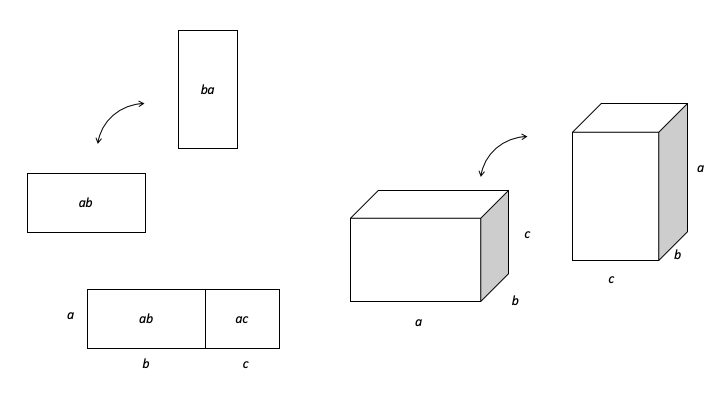
\includegraphics[scale=0.4]{img/geometric-arithmetic.png}
  % \captionsetup{labelformat=empty}
 \caption{Geometric explanation for arithmetic laws}
 \label{fig:geometric-arithmetic}
\end{figure}

\item Define square for natural number $()^2$ with $foldn$;

We can define square from the iterative relation $(n+1)^2 = n^2 + 2n + 1$

\[
()^2 = 2nd \cdot foldn\ (0, 0)\ h
\]

Where $h$ accepts a pair $(i, s)$, which means the number $i$ and its square $s$. It increase $i$ by 1, then use the iterative relation to calculate the next square.

\[
h\ (i, s) = (i + 1, s + 2i + 1)
\]

\item Define $()^m$ with $foldn$, which gives the $m$-power of a natural number;

One simple method is to re-use the definition of $m^{()} = foldn(1, (\cdot m))$ in chapter 1 for $()^m$

\[
()^m = 2nd \cdot foldn\ (0, 0)\ h
\]

where

\[
h\ (i, b) = (i + 1, (i + 1)^m)
\]

It looks a bit strange, as all the intermediate results are dropped. Another method is to leverage the Newton's binomial theorem:

\[
(n + 1)^m = n^m + \binom{m}{1} n^{m-1} + ... + \binom{m}{m-1} n + 1
\]

Hence we can establish the iterative relation:

\[
(n)^m = 2nd(foldn\ (1, 1)\ h\ (n - 1))
\]

where

\[
h (i, x) = (i + 1, C \cdot X)
\]

The $C \cdot X$ is the dot product between binomial coefficients and the powers: $C \cdot X = \sum c_j x_j$. The powers can be calculated by repeatedly dividing $x$ by $i$, and the binomial coefficients can be iterated from the Pascal triangle. Below is an example program that put them together:

\lstset{language=Haskell
    , frame=single
}
\begin{lstlisting}
exp m n = snd $ foldn (1, 1) h (n - 1) where
  cs = foldn [1] pascal m
  h (i, x) = (i + 1, sum $ zipWith (*) cs xs) where
    xs = take (m + 1) $ iterate (`div` i) x

pascal = gen [1] where
  gen cs (x:y:xs) = gen ((x + y) : cs) (y:xs)
  gen cs _ = 1 : cs
\end{lstlisting} %$

\item Define sum of odd numbers with $foldn$, what sequence does it produce?


1 + 3 + 5 + ... can be defined with $foldn$ as $2nd \cdot foldn\ (1, 0)\ h$, where:

\[
h\ (i, s) = (i + 2, s + i)
\]

As shown in the figure below this exercise in chapter 1, the sum of odd numbers is always square number.

\item There is a line of holes in the forest. A fox hides in one hole. It moves to the next hole every day. If we can check only one hole a day, is there a way to catch the fox? Prove this method works. What if the fox moves more than one hole a day?

No matter which hole the fox hides in, we only examine the odd numbered ones 1, 3, 5, ... It can ensure us always catch the fox. Observe the below table:

\btab{c|c|c|c|c}
1 & 3 & 5 & ... & 2m - 1 \\
\hline
m & m + 1 & m + 2 & ... & 2m - 1 \\
\etab

Suppose the fox hides in the hole number $m$, solving equation $m + k = 2k + 1$ gives that, after $k = m -1$ days, we will examine the hole number $2m - 1$, while the fox moves exactly to it. Below $foldn$ program demonstrates this process:

\[
\begin{array}{l}
fox\ m = foldn\ (1, m)\ h\ (m - 1) \\
\text{where}: h\ (c, f) = (c + 2, f + 1) \\
\end{array}
\]

If the fox hides at hole number $p$, and moves $q$ holes everyday, we can denote such pair as $(p, q)$, then map them to the natural numbers with the method we introduced in chapter 6 about infinity. With this method, we can enumerate all $(p, q)$ combinations and catch the fox.

\item What does the expression $foldr(nil, cons)$ define?

It defines the list itself.

\item Read in a sequence of digits (string of digit numbers), convert it to decimal with $foldr$. How to handle hexadecimal digit and number? How to handle the decimal point?

If the lowest digit is on the left, and the highest digit on the right in the input list, we can convert it as below:

\[
foldr\ (c\ d \mapsto 10d + c)\ 0
\]

However, if the lowest digit is on the right, and the elements in the list are characters but not digit, then we need adjust it to:

\[
1st \cdot foldr\ (c, (d, e) \mapsto ((toInt\ c)e + d, 10e))\ (0, 1)
\]

We can make it process the hexadecimal numbers by replacing 10 to 16 in this definition. When meets the decimal point, we can divided $d$, the result so far, by $e$ to calculate the fractional part value.

\[
1st \cdot foldr\ h\ (0, 1)
\]

where

\[
h\ (c, (d, e)) = \begin{cases}
c = '.' & (d / e, 1) \\
\text{otherwise} & ((toFloat\ c)e + d, 10e) \\
\end{cases}
\]

\item Jon Bentley gave the maximum sum of sub-vector puzzle in {\em Programming Pearls}. Given an integer list $\{x_1, x_2, ..., x_n\}$, find the sub-section $i, j$, that maximize the sum of $x_i + x_{i+1} + ... + x_j$. Solve it with $foldr$.

If all numbers are positive, then the maximum sum must be sum of the whole list. This is because the adding is monotone increasing upon positive numbers. If all numbers are negative, then the maximum sum should be zero, which is the sum of empty list. For any sub-list, the sum increases when add a positive number, while it decreases when add a negative number. We can maintain two things during folding: one is the maximum sum of sub-list found so far $S_m$, the other is the sum of the sub-list till the current number being examined $S$. By adding the next element, if $S$ exceeds $S_m$, it means we found a larger sub-list sum. Hence we replace $S_m$ with $S$; If $S$ becomes negative, it means we complete the previous sub-list, and should start a new sub-list.

\blre
max_s & = & 1st \cdot foldr\ f\ (0, 0) \\
\text{where}: & & f\ x\ (S_m, S) = (S_m', S') \\
& & \text{where in $f$}:  S' = max(0, x + S), S_m' = max(S_m, S') \\
\elre

If want to return the sub-list together with the maximum sum, we can maintain two pairs $P_m$ and $P$ during folding, each pair contains the sum and the sub-list $(S, L)$.

\blre
max_s & = & 1st \cdot foldr\ f\ ((0, []), (0, [])) \\
\text{where}: & & f\ x\ (P_m, (S, L)) = (P_m', P') \\
& & \text{where in $f$}:  P' = max((0, []), (x + S, x:L)), P_m' = max(P_m, P') \\
\elre

\item The longest sub-string without repeated characters. Given a string, find the longest sub-string that there are no repeated characters in it. For example, the answer for string ``abcabcbb'' is ``abc''. Solve it with $foldr$.

We give two methods. One solution is to maintain the longest sub-string without repeated characters found during folding, record and check if the character $c$ has met before and its last appeared position. If $c$ never occurred, or it appears before the current sub-string we are examining, then we append it to the current sub-string, and compare it with the longest one we've found so far. Otherwise, it means the current sub-string contains a repeated character, we need go back to the its last occurred position, move ahead one, then reset the search.

\[
longest(S) = fst2 \cdot foldr\ f\ (0, |S|, |S|, \varnothing)\ zip(\{1, 2, ...\}, S)
\]

Where folding starts from a 4 elements tuple, which contains the length of the longest sub-string we found so far, the right boundary of the longest sub-string, the right boundary of the current sub-string, and a map recorded the last occurred position for different characters. Function $fst2$ extract the first two elements from the tuple as result. To obtain the position of each character easily during folding, we $zip$ the string $S$ and natural number sequence together. The most critical function $f$ is defined as below:

\[
f\ (i, c)\ (n_{max}, e_{max}, e, Idx) = (n_{max}', e_{max}', e', Idx[c] = i)
\]

where:

\[ \begin{array}{l}
n_{max}' = max(n_{max}, e' - i + 1) \\
e' = \begin{cases}
  c \notin Idx: & e \\
  Idx[c] = j: & min(e, j - 1) \\
  \end{cases} \\
e_{max}' = \begin{cases}
  e' - i + 1 > n_{max}: & e' \\
  \text{otherwise}: & e_{max} \\
  \end{cases} \\
\end{array} \]

We record ending position because $foldr$ starts from right. While the traditional way starts from the left, for example:

\begin{algorithmic}
\Function{Longest}{$S$}
  \State $Idx \gets \varnothing$
  \State $n_{max} \gets 0, s_{max} \gets 0, s \gets 0$
  \For{$i \in \{0, 1, ... |S|\}$}
    \If{$S[i] \in Idx$}
      \State $j \gets Idx[S[i]]$
      \State $s = max(s, j + 1)$
    \EndIf
    \If{$i - s + 1 > n_{max}$}
      \State $s_{max} \gets s$
    \EndIf
    \State $n_{max} \gets max(n_{max}, i - s + 1)$
    \State $Idx[S[i]] = i$
  \EndFor
  \State \Return $S[s_{max} ... s_{max} + n_{max}]$
\EndFunction
\end{algorithmic}

The second method is a number theory solution by leveraging prime numbers. We map each unique character $c$ to a prime number $p_c$. For any string $S$, we can calculate a product of prime numbers mapped from its characters:

\[
P = \displaystyle \prod_{c \in S} p_c
\]

Therefore, for any new character $c'$, we can check whether the corresponding prime number $p'$ divides $P$ or not to know if $c'$ appears in $S$. Based on this fact, we can design an algorithm, it maintain the product of primes during folding. When there is a character, its corresponding prime number divides the product, we then find a repeated character. We need drop off the part containing the repeated character and go on folding. During this process, we also need update the longest sub-string.

\[
longest = fst \cdot foldr\ f\ ((0, []), (0, []), 1)
\]

Where the folding starts from a three element tuple. The first two are pairs, represent the longest sub-string (its length and content), and the current sub-string. The last one in the tuple is the product of primes, starts from 1. Function $f$ is defined as the following:

\[
f\ c\ (m, (n, C), P) = \begin{cases}
  p_c | P : & update(m, (n + 1, c : C), p_c \times P) \\
  \text{otherwise}: & update(m, (|C'|, C'), \displaystyle \prod_{x \in C'} p_x) \\
\end{cases}
\]

where:

\[ \begin{array}{l}
update(a, b, P) = (max(a, b), b, P) \\
C' = c : takeWhile\ (\neq c)\ C \\
\end{array} \]

\item {In the fold definition of Fibonacci numbers, the successor is computed as $(m', n') = (n, m + n)$. It is essentially matrix multiplication:
\[
\begin{pmatrix} m' \\ n' \end{pmatrix} =
\begin{pmatrix} 0 & 1 \\ 1 & 1 \end{pmatrix}
\begin{pmatrix} m \\ n \end{pmatrix}
\]
Where it starts from $(0, 1)^T$. Then the Fibonacci numbers is isomorphic to natural numbers under the matrix multiplication:
\[
\begin{pmatrix}F_n \\ F_{n+1} \end{pmatrix} = \begin{pmatrix} 0 & 1 \\ 1 & 1 \end{pmatrix}^n\begin{pmatrix} 0 \\ 1 \end{pmatrix}
\]
Write a program to compute the power of 2-order square matrix, and use it to give the $n$-th Fibonacci number.}

First we need define multiplication for square matrix of order 2, and the multiplication between the square matrix and vector:

\[
\begin{pmatrix}
a_{11} & a_{12} \\
a_{21} & a_{22} \\
\end{pmatrix}
\times
\begin{pmatrix}
b_{11} & b_{12} \\
b_{21} & b_{22} \\
\end{pmatrix}
=
\begin{pmatrix}
a_{11} b_{11} + a_{12} b_{21} & a_{11} b_{12} + a_{12} b_{22} \\
a_{21} b_{11} + a_{22} b_{21} & a_{21} b_{12} + a_{22} b_{22} \\
\end{pmatrix}
\]

and

\[
\begin{pmatrix}
a_{11} & a_{12} \\
a_{21} & a_{22} \\
\end{pmatrix}
\times
\begin{pmatrix}
b_{1} \\
b_{2} \\
\end{pmatrix}
=
\begin{pmatrix}
a_{11} b_{1} + a_{12} b_{2} \\
a_{21} b_{1} + a_{22} b_{2} \\
\end{pmatrix}
\]

When calculate the $n$-th power of $M^n$, we need not repeat multiplication $n$ times. If $n = 4$, we can first calculate $M^2$, then multiply the result to itself to obtain $(M^2)^2$. There are total two times of multiplication; If $n = 5$, we only need compute $M^4 \times M$, hence there are three times of multiplication. We can recursively fast compute the exponential based on $n$'s parity.

\[
M^n = pow(M, n, I)
\]

Where $I$ is the identical square matrix of order 2: $\displaystyle \begin{pmatrix} 1 & 0 \\ 0 & 1\end{pmatrix}$, and the function $pow$ is defined as below:

\[
pow(M, n, A) = \begin{cases}
n = 0: & A \\
n\text{is even}: & pow(M \times M, \dfrac{n}{2}, A) \\
\text{otherwise}: & power(M \times M, \lfloor \dfrac{n}{2} \rfloor, M \times A)\\
\end{cases}
\]

In fact, we can represent $n$ in binary format, then perform folding on these 0, 1 bits to fast compute $M^n$.

\end{enumerate}

\section{Recursion}

\begin{enumerate}
\item {The Euclidean algorithm described in this section is in recursive manner. Try to eliminate recursion, implement it and the extended Euclidean algorithm only with loop.}

The classic Euclidean algorithm is tail recursive, it can be convert to loop easily:

\begin{algorithmic}
\Function{GCM}{$a, b$}
\While{$b \neq 0$}
  \State $a, b \gets b, a \bmod b$
\EndWhile
\State \Return $a$
\EndFunction
\end{algorithmic}

However, it's a bit hard to convert the extended Euclidean algorithm. Let us see three sequences $r, s, t$:

\[\begin{array}{l}
r_0 = a, r_1 = b \\
s_0 = 1, s_1 = 0 \\
t_0 = 0, t_1 = 1 \\
 ...  ... \\
r_{i+1} = r_{i-1} - q_{i} r_{i}, \text{where}: q_{i} = \lfloor r_{i} / r_{i-1} \rfloor \\
s_{i+1} = s_{i-1} - q_{i} s_{i} \\
t_{i+1} = t_{i-1} - q_{i} t_{i} \\
... ...\\
\end{array}\]

Obviously, when $r_{k+1} = 0$, the sequences terminate. We also know from Euclidean algorithm that at this time:

\[
gcm(a, b) = gcm(r_{k-1}, r_{k}) = gcm(r_k, 0) = r_{k}
\]

The more important fact is that, at this time, the following Bézout's identity holds:

\[
gcm(a, b) = r_{k} = a s_{k} + b t_{k}
\]

\begin{proof}
We prove it with mathematical induction. First for 0 and 1:

\blre
0: & r_0 = a & a s_0 + b t_0 = a \cdot 1 + b \cdot 0 = a \\
1: & r_1 = b & a s_1 + b t_1 = a \cdot 0 + b \cdot 1 = b \\
\elre

Next suppose $r_{i-1} = a s_{i-1} + b t_{i-1}$ and $r_{i} = a s_{i} + b t_{i}$ hold, for $i + 1$ case:

\bre
r_{i+1} & = & r_{i-1} - q_{i} r_{i} & \text{sequence definition} \\
       & = & (a s_{i-1} + b t_{i-1}) - q_{i} (a s_{i} + b t_{i}) & \text{induction assumption} \\
       & = & a (s_{i-1} - q_{i} s_{i}) + b (t_{i-1} - q_{i} t_{i}) & \text{rearrange} \\
       & = & a s_{i+1} + b t_{i+1} & \text{sequence definition} \\
\ere

Hence the sequences satisfy Bézout's identity at any time.
\end{proof}

With this fact, we can obtain the non-recursive realization for extended Euclidean algorithm:

\begin{algorithmic}
\Function{Ext-GCM}{$a, b$}
  \State $s', s \gets 0, 1$
  \State $t', t \gets 1, 0$
  \While{$b \neq 0$}
    \State $q, r \gets \lfloor a / b \rfloor, a \bmod b$
    \State $s', s \gets s - q s', s'$
    \State $t', t \gets t - q t', t'$
    \State $a, b \gets b, r$
  \EndWhile
  \State \Return $(a, s, t)$
\EndFunction
\end{algorithmic}

\item {Most programming environments require integers for modular operation. However, the length of segment isn't necessarily integer. Implement a modular operation that manipulates segments. What's the efficiency of it?}

Consider the compass and straightedge construction, we can use compass to intercept segment to obtain the modular result.

\begin{algorithmic}
\Function{mod}{$a, b$}
  \While{$b < a$}
    \State $a \gets a - b$
  \EndWhile
  \State \Return $a$
\EndFunction
\end{algorithmic}

It's efficiency is linear obviously. To optimize it, we introduce a lemma:

\begin{lemma}[Recursive remainder lemma] % recursive remainder lemma
If $r = a \bmod 2b$, then:
\[
a \bmod b = \begin{cases}
r \leq b: & r \\
r > b: & r - b \\
\end{cases}
\]
\end{lemma}

With this lemma, we can speed up the modular operation to logarithmic:

\[
a \bmod b \begin{cases}
a \leq b: & a \\
a - b \leq b: & a - b \\
\text{otherwise}: & \begin{cases}
  a' \leq b: & a', \text{where} a' = a \bmod (b + b) \\
  a' > b: & a' - b \\
  \end{cases} \\
\end{cases}
\]

Inspired by Fibonacci numbers, Robot Floyd, and Donald Knuth managed to eliminate the recursion in this algorithm, hence obtained a pure iterative modular operation:

\begin{algorithmic}
\Function{mod}{$a, b$}
  \If{$a < b$}
    \State \Return $a$
  \EndIf
  \State $c \gets b$
  \While{$c \leq a$}
    \State $c, b \gets (b + c, c)$ \Comment{Increase $c$ like Fibonacci numbers}
  \EndWhile
  \While{$b \neq c$}
    \State $c, b \gets (b, c - b)$ \Comment{Decrease $c$ back}
    \If{$c <= a$}
      \State $a \gets a - c$
    \EndIf
  \EndWhile
  \State \Return $a$
\EndFunction
\end{algorithmic}

\item {In the proof of Euclidean algorithm, we mentioned ``Remainders are always less than the divisor. We have $b > r_0 > r_1 > r_2 > ... > 0$. As the remainder can not less than zero, and the initial magnitude is finite, the algorithm must terminate.'' Can $r_{n}$ infinitely approximate zero, but not be zero? Does the algorithm always terminate? What does the precondition that $a$ and $b$ are commensurable ensure?}

For the commensurable magnitudes, we can use the {\em Well-ordering principle} to show that the Euclidean algorithm must terminate. According to the well-ordering principle, every none empty set of natural numbers has the minimum number. This property can be extended to set of integers, rationals, or even to the finite, none empty sub-set of real numbers. From the definition of commensurable, we know the remainders form a finite set.

\item {For the binary linear Diophantine equation $ax + by = c$, let $x_1, y_1$ and $x_2, y_2$ are two pairs of solution. Proof that the minimum of $|x_1 - x_2|$ is $b/gcm(a, b)$, and the minimum of $|y_1 - y_2|$ is $a/gcm(a, b)$}

Let the greatest common divisor of $a$ and $b$ be $g = gcm(a, b)$. If $x_0, y_0$ is a pair of solution to the Diophantine equation $ax + by = c$, then the following $x, y$ is also a pair of solution:

\[
\begin{dcases}
  x = x_0 - k \dfrac{b}{g} \\
  y = y_0 + k \dfrac{a}{g}
\end{dcases}
\]

It's easy to verify this fact:

\blre
ax + by & = & a (x_0 - k \dfrac{b}{g}) + b (y_0 - k \dfrac{a}{g}) \\
        & = & a x_0 + b y_0 - a k \dfrac{b}{g} + b k \dfrac{a}{g} \\
        & = & c - 0 = c
\elre

We next prove that, every solution can be expressed in this form. Let $x, y$ be an arbitrary pair of solution, we have $ax + by = c$ and $a x_0 + b y_0 = c$ both hold, therefore:

\[
a (x - x_0) + b (y - y_0) = c - c = 0
\]

Divide both sides with the greatest common divisor of $a$ and $b$. It gives:

\[
\dfrac{a}{g} (x - x_0) + \dfrac{b}{g} (y - y_0) = 0
\]

\[
\dfrac{b}{g} (y - y_0)  = - \dfrac{a}{g} (x - x_0)
\]

Note that the left side can be divided by $\dfrac{b}{g}$, hence it must divide the right side too. But since $(\dfrac{a}{g}, \dfrac{b}{g}) = 1$, they are co-prime, hence $\dfrac{b}{g}$ must divide $(x - x_0)$. Let

\[
x - x_0 = k \dfrac{b}{g}, \text{for some}\ k \in \pmb{Z}
\]

Therefore

\[
x = x_0 + k \dfrac{b}{g}
\]

Substitute it back to above equation, we obtain:

\[
y = y_0 - k \dfrac{a}{g}
\]

Hence proved every pair of solution is in this form. Obviously, for any two such pairs, the minimized difference is obtained when $k = 1$. It means the minimum of $|x_1 - x_2|$ is $b/gcm(a, b)$, and the minimum of $|y_1 - y_2|$ is $a/gcm(a, b)$.

\item {For right pentagon with side of 1, how long is the diagonal? Proof that in the pentagram shown in this chapter, the segment $AC$ and $AG$ are incommensurable. What's their ratio in real number?}

Paul Lockhart gives a beautiful method in his {\em Measurement}\cite{Lockhart2012}. As shown in figure \ref{fig:pentagram-unit}, we can divide the regular pentagram into three triangles. It's easy to show that triangle $A$ and $B$ are congruent, and they are similar to triangle $C$ (can you prove it?). If the length of the pentagram side is 1, let the diagonal length be $d$, then the base of triangle $C$ is 1, and its two hypotenuses both are $d - 1$. From the similar triangles, we have:

\[
  1 / d = (d - 1) / a
\]

Solving this quadratic equation gives $d = \dfrac{\sqrt{5} + 1}{2}$. We drop the other solution $d = \dfrac{\sqrt{5} - 1}{2}$ as it is shorter than the side (in fact, it is the length of the hypotenuse of the smaller triangle $C$).

For the segment AC and AG in the figure of this chapter, according to the 3 triangles we divided, they are actually the side and the diagonal of the pentagram. Suppose they are commensurable, then the base and hypotenuse of the smaller triangle are commensurable. Hence in the recursive inner pentagram star, the side and diagonal are also commensurable. We can repeat this process infinitely without end. Therefore, our assumption cannot hold. The side and diagonal are incommensurable. Written in decimals, it is about 0.6180339887498949...

\begin{figure}[htbp]
 \centering
 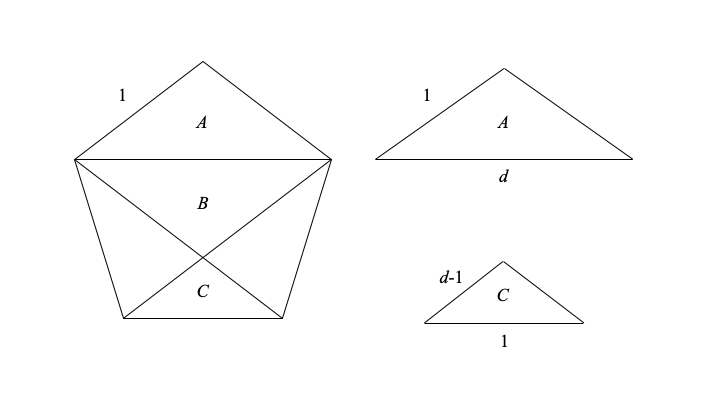
\includegraphics[scale=0.4]{img/pentagram-unit.png}
 \captionsetup{labelformat=empty}
 \caption{The unit regular pentagram}
 \label{fig:pentagram-unit}
\end{figure}

\item {Use $\lambda$ conversion rules to verify $tail\ (cons\ p\ q) = q$。}

The $\lambda$ expressions for $cons$ and $tail$ are:

\[
\begin{array}{rcl}
cons & = & a \mapsto b \mapsto f \mapsto f\ a\ b \\
tail & = & c \mapsto c\ (a \mapsto b \mapsto b)
\end{array}
\]

From the two definitions, we can verify $tail\ (cons\ p\ q) = q$ holds.

\[
\begin{array}{rcl}
tail\ (cons\ p\ q) & = & (c \mapsto c\ (a \mapsto b \mapsto b))\ (cons\ p\ q) \\
                   & \xrightarrow{\beta} & (cons\ p\ q)\ (a \mapsto b \mapsto b) \\
                   & = & ((a \mapsto b \mapsto f \mapsto f\ a\ b)\ p\ q)\ (a \mapsto b \mapsto b) \\
                   & \xrightarrow{\beta} & ((b \mapsto f \mapsto f\ p\ b)\ q)\ (a \mapsto b \mapsto b) \\
                   & \xrightarrow{\beta} & (f \mapsto f \mapsto f\ p\ q)\ (a \mapsto b \mapsto b) \\
                   & \xrightarrow{\beta} & (a \mapsto b \mapsto b)\ p\ q \\
                   & \xrightarrow{\beta} & (b \mapsto b)\ q \\
                   & \xrightarrow{\beta} & q
\end{array}
\]

\item {We can define numbers with $\lambda$ calculus. The following definition is called Church numbers:

\[
\begin{array}{r@{\quad:\quad}l}
0 & \lambda f . \lambda x . x \\
1 & \lambda f . \lambda x . f\ x \\
2 & \lambda f . \lambda x . f\ (f\ x) \\
3 & \lambda f . \lambda x . f\ (f\ (f\ x)) \\
  & ...
\end{array}
\]
Define the addition and multiplication operators for the Church numbers with what we introduced in chapter 1.
}

For natural number $n$, the meaning as a Church number is to apply function $f$ to $x$ by $n$ times. Let's define successor function first:

\[
succ = \lambda n . \lambda f . \lambda x . f\ (n\ f\ x)
\]

It means $f^{n+1}(x)) = f(f^n(x))$. Then we can define addition as:

\[
plus = \lambda m . \lambda n . \lambda f . \lambda x . m\ f\ (n\ f\ x)
\]

Which means $f^{m + n}(x) = f^m(f^n(x))$. While the multiplication is defined as:

\[
mul = \lambda m . \lambda n . \lambda f . \lambda x . m\ (n\ f)\ x
\]

It means $f^{m n} = (f^n)^m(x)$.

\item {The following defines the Church Boolean values, and the relative logic operators:

\[
\begin{array}{r@{\quad:\quad}l}
\textbf{true} & \lambda x . \lambda y . x \\
\textbf{false} & \lambda x . \lambda y . y \\
\textbf{and} & \lambda p . \lambda q . p\ q\ p \\
\textbf{or} & \lambda p . \lambda q . p\ p\ q \\
\textbf{not} & \lambda p . p\ \textbf{false}\ \textbf{true}
\end{array}
\]

where \textbf{false} is defined as same as the Church number 0. Use the $\lambda$ conversion rules to prove that: \textbf{and}\ \textbf{true}\ \textbf{false} = \textbf{false}. Please give the definition of if ... then ... else ... expression with the $\lambda$ calculus.
}

\blre
and\ true\ false & = & (\lambda p . \lambda q . p\ q\ p)\ true\ false \\
 & \xrightarrow{\beta} & true\ false\ true \\
 & = & (\lambda x . \lambda y . x)\ false\ true \\
 & \xrightarrow{\beta} & false \\
\elre

if ... then ... else ... expression can be defined as: $\lambda p . \lambda a . \lambda b . p\ a\ b$

\item {Define the abstract $mapt$ for binary trees without of using $foldt$.}

\[ \begin{cases}
mapt(f, nil) & = nil \\
mapt(f, node(l, x, r)) & = node(mapt(f, l), f(x), mapt(f, r)) \\
\end{cases}\]

\item {Define a function $depth$, which counts for the maximum depth of a binary tree.}

\[
depth = foldt(one, x, y \mapsto 1 + max(x, y), 0)
\]

Where $one$ is a constant function. It always returns 1. i.e. $one = x \mapsto 1$.

\item {Someone thought the abstract fold operation for binary tree $foldt$, should be defined as the following:
\[
\begin{array}{l}
foldt(f, g, c, nil) = c \\
foldt(f, g, c, node(l, x, r)) = foldt(f, g, g(foldt(f, g, c, l), f(x)), r)
\end{array}
\]
That is to say $g : (B \times B) \to B$ is a binary operation like add. Can we use this $foldt$ to define $mapt$?}

This $foldt$ cannot define tree mapping. A tree should be mapped to another tree with the same structure. Each value in the tree is sent to another value. Note the type of $f$ is $f : A \to B$, it send the element of type $A$ in the tree to type $B$. While the type of $g$ is $g : (B \times B) \to B$, it only maps values of $B$, but cannot preserve the tree structure.

\item {The binary search tree (BST) is a special tree that the type A is comparable. For any none empty $node(l, k, r)$, all elements in the left sub-tree $l$ are less than $K$, and all elements in the right sub-tree $r$ are greater than $k$. Define function $insert(x, t) : (A \times Tree\ A) \to Tree\ A$ that inserts an element into the tree.}

\[ \begin{cases}
insert(x, nil) = node(nil, x, nil) \\
insert(x, node(l, k, r)) = \begin{cases}
  x < k: & node(insert(x, l), k, r) \\
  \text{otherwise}: & node(l, k, insert(x, r)) \\
\end{cases} \\
\end{cases}\]

\item {Can we define the mapping operation for multi-trees with folding? If not, how should we modify the folding operation?}

Similar to above exercise, we need modify the folding definition for multi-tree to preserve the tree structure:

\[
\begin{cases}
foldm(f, g, c, nil) & = c \\
foldm(f, g, c, node(x, ts)) & = g(f(x), map(foldm(f, g, c), ts)) \\
\end{cases}
\]

Where $map$ applies to list. With this tree folding tool, we can define multi-tree map as below:

\[
mapm(f) = foldm(f, node, nil)
\]

\end{enumerate}

\section{Symmetry}

\begin{enumerate}
\item {Do all the even numbers form a group under addition?}

Yes, even numbers form a group under addition. Even number add even number, the result is still even. Add is associative. The unit is zero. The inverse of a number is its negate.

\item {Can we find a subset of integers, that can form a group under multiplication?}

The subset $\{ -1, 1 \}$ form a group under multiplication. The unit is 1. Every element is the reverse of itself.

\item {Do all the positive real numbers form a group under multiplication?}

Yes. Positive real numbers are close under multiplication. The unit is 1. For each number $r$, the reverse is $1/r$.

\item {Do integers form a group under subtraction?}

No, integers cannot form a group under subtraction. This is because subtraction is not associative. for e.g. (3 - 2) - 1 = 0, while 3 - (2 - 1) = 2.

\item {Find an example of group with only two elements.}

As shown in previous exercise, set ${-1, 1}$ forms a group under addition. Another example is Boolean values $\{T, F\}$, they form a group under logic exclusive or (xor). The logic exclusive or is closed and associative. The unit is $F$, because every element exclusive or $F$ gives itself. And every element is the reverse of itself.

\item {What is the identity element for Rubik cube group? What is the inverse element for $F$?}

The unit for the Rubik cube group is the identity transform, which keep any state unchanged. The reverse of $F$ is $F'$, which rotate the face side 90 degree counterclockwise.

\item {The set of Boolean values \{True, False\} forms a monoid under the logic or operator $\lor$. It is called `Any' logic monoid. What is the identity element for this monoid?}

False

\item {The set of Boolean values \{True, False\} forms a monoid under the logic and operator $\land$. It is called `All' logic monoid. What is the identity element for this monoid?}

True

\item {For the comparable type, when compare two elements, there can be three different results. We abstract them as $\{<, =, >\}$\footnote{Some programming languages, such as C, C++, Java use negative number, zero, and positive number to represent these three results. In Haskell, they are GT, EQ, and LE respectively.}. For this set, we can define a binary operation to make it a monoid. What is the identity element for this monoid?}

Define the binary operation as:

\blre
< \circ\ x & = & < \\
= \circ\ x & = & x \\
> \circ\ x & = & > \\
\elre

Where $x$ is any element among the three. These three relations form a monoid. The unit is $=$.

\item {Prove that the power operation for group, monoid, and semigroup is commutative: $x^mx^n = x^nx^m$}

In order to prove the commutative law, we first use mathematical induction to prove a lemma: $x^n x = x x^n$. For group and monoid, when $n = 0$:

\[
x^0 x = e x = x = x e = x x^0
\]

As there is no unit in semigroup, we start from $n = 1$:

\[
x^1 x = x x = x x^1
\]

Suppose for $n$, $x^n x = x x^n$ holds, then for $n + 1$:

\bre
x^{n + 1} x & = & (x x^n) x & \text{recursive definition of power} \\
  & = & x (x^n x) & \text{associative} \\
  & = & x (x x^n) & \text{induction hypothesis} \\
  & = & x x^{n + 1} & \text{recursive definition of power} \\
\ere

With this lemma, we use mathematical induction again to prove the commutativity for power operation. For group and monoid, when $n = 0$, we have:

\bre
x^m x ^ 0 & = & x^m e & \text{definition of 0-th power} \\
  & = & x^m & \text{definition of unit} \\
  & = & e x^m & \text{definition of unit} \\
  & = & x^0 x^m & \text{definition of 0-th power} \\
\ere

Because semigroup does not have unit, we start from $n = 1$:

\bre
x^m x ^ 1 & = & x^m x & \text{definition of 1-st power} \\
  & = & x x^m & \text{the lemma} \\
  & = & x^1 x^m & \text{definition of 1-st power} \\
\ere

Suppose the commutativity law $x^mx^n = x^nx^m$ holds for $n$, then for $n + 1$ case:

\bre
x^m x^{n+1} & = & x^m (x x^n) & \text{recursive definition of power} \\
  & = & (x^m x) x^n & \text{associative law for multiplication} \\
  & = & x x^m x^n & \text{the lemma} \\
  & = & x (x^m x^n) & \text{associative law for multiplication} \\
  & = & x (x^n x^m) & \text{induction hypothesis} \\
  & = & (x x^n) x^m & \text{associative law for multiplication} \\
  & = & x^{n+1} x^m & \text{recursive definition of power} \\
\ere

\item {Is the odd even test function homomorphic between the integer addition group $(Z,+)$ and the Boolean logic-and group $(Bool, \land)$? What about the group of integers without zero under multiplication?}

To test homomorphic, we need verify two things: 1, whether it is surjective; 2, whether $f(a) f (b) = f(a \cdot b)$ holds. Although the odd-even test is surjective, there is a negative case:

$a, b$ are all odd, i.e. $odd(a) = odd(b) = True$. Their sum is even, $odd(a + b) = False$. However, the logic and result is $odd(a) \land odd(b) = True \neq odd(a + b) = False$.

Hence they are not homomorphic.

While the multiplicative group of integers without zero is homomorphic with the logic and group. We can verify all the three cases:

  \begin{itemize}
  \item $a, b$ are all odd, i.e. $odd(a) = odd(b) = True$. Their product $ab$ is still odd: $odd(ab) = True$. Hence, $odd(a) \land odd(b) = odd(ab)$;
  \item $a, b$ are all even, i.e. $odd(a) = odd(b) = False$. Their product $ab$ is still even: $odd(ab) = False$. Hence, $odd(a) \land odd(b) = odd(ab)$;
  \item $a, b$ are old and even respectively. Let $odd(a) = True, odd(b) = False$. Their product $ab$ is even: $odd(ab) = False$. Hence, $odd(a) \land odd(b) = odd(ab)$.
  \end{itemize}

Therefore, they are homomorphic.

\item {Suppose two groups $G$ and $G'$ are homomorphic. In $G$, the element $a \to a'$. Is the order of $a$ same as the order of $a'$?}

Their orders are same. To prove it, let the image of unit $e$ be $e'$, the homomorphism is $f$. Denote the order of $a$ is $n$, i.e. $a^n = e$.

On one hand:
\[
f(a^n) = f(e) = e'
\]

On the other hand, according to the definition of homomorphism:

\bre
f(a^n) & = & f(a) f(a) ... f(a) & \text{total $n$} \\
  & = & a' a' ... a' & \text{total $n$} \\
  & = & (a')^n
\ere

Summarize the above two results, we have $(a')^n = e'$. Hence the order of $a$ and $a'$ are same.

\item {Prove that the identity element for transformation group must be identity transformation.}

Suppose the unit transformation is $\epsilon': a \to a^{\epsilon'} = \epsilon'(a)$. According to the definition of unit, for any transformation $\tau$, $\epsilon' \tau = \tau$ holds, i.e.

\[
\begin{array}{l}
\tau: a \to a^\tau \\
\epsilon' \tau: a \to (a^{\epsilon'})^\tau \\
\end{array}
\]

Therefore, $a^{\epsilon'} = a = \epsilon'(a)$, $\epsilon'$ is identity transformation.

\item{List all the elements in $S_4$.}

(1);

(12), (34), (13), (24), (14), (23);

(123), (132), (134), (143), (124), (142), (234), (243);

(1234), (1243), (1324), (1342), (1423), (1432);

(12)(34), (13)(24), (14)(23)。

There are total $4! = 24$ elements.

\item {Express all the elements in $S_3$ as the product of cyclic forms.}

\btab{c|c|c|c|c|c|c}
permutation & 123 & 213  & 132  & 321  & 231   &  312\\
\hline
cyclic notation & (1) & (12) & (23) & (13) & (123) & (132)\\
\etab

\item{Write a program to convert the product of $k$-cycles back to permutation.}

\begin{algorithmic}
\Function{Permute}{$C, n$}
  \State $\pi \gets [1, 2, ..., n]$
  \For{$c \in C$}
    \State $j \gets c[1]$
    \State $m \gets |c|$
    \For{$i \gets 2$ to $m$}
      \State $\pi[j] \gets c[i]$
      \State $j \gets c[i]$
    \EndFor
    \State $\pi[c[m]] \gets c[1]$
  \EndFor
  \State \Return $\pi$
\EndFunction
\end{algorithmic}

\item{What symmetries for what shape are defined by the symmetric group $S_4$?}

It defines the symmetry of a tetrahedron. A tetrahedron has four vertex corners, each has an axis. Rotation around such axis by 120 and 240 degree is symmetric. Connect the middle point of every two opposite edges also gives an axis. There are total 3 such axes, each one is reflective symmetric. Include the identity transformation, there are total $2 \times 4 + 3 + 1 = 12$ symmetries. They are corresponding to the elements in $S_4$.

\begin{figure}[htbp]
 \centering
 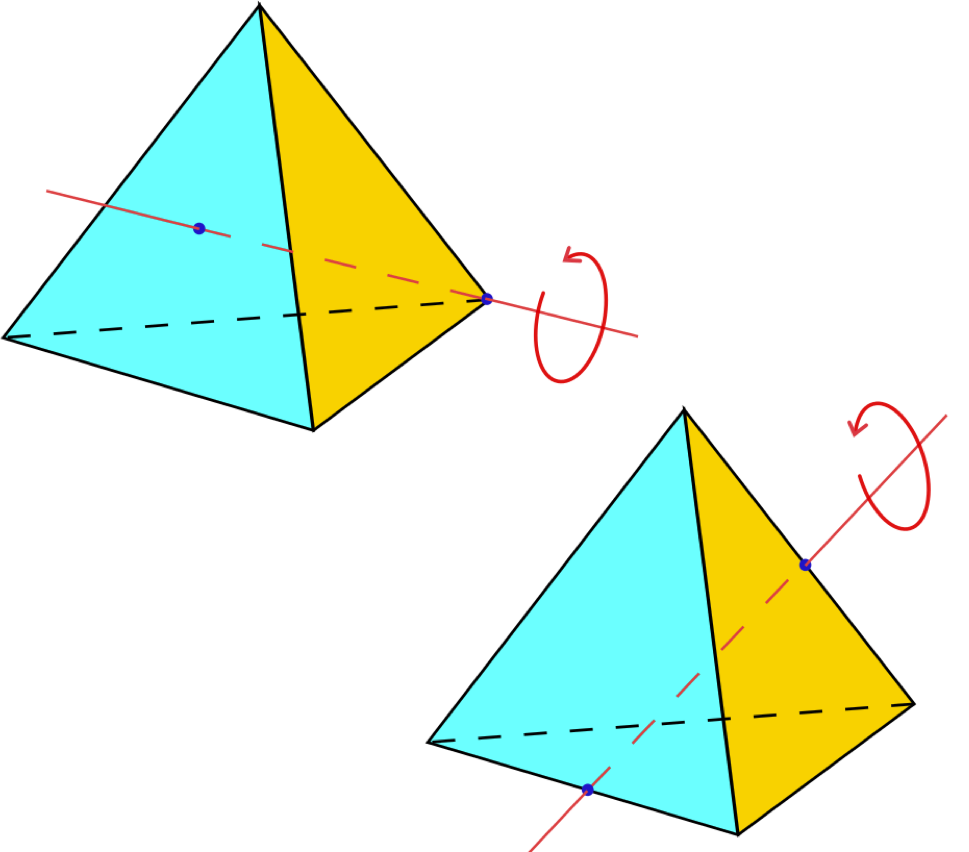
\includegraphics[scale=0.5]{img/tetrahedron.png}
 %\captionsetup{labelformat=empty}
 \caption{The rotation and reflection axes}
 \label{fig:tetrahedron}
\end{figure}

\item {Proof that cyclic groups are abelian.}

Let the generator be $a$. For any two elements, express them as the power of $a$, i.e. $a^p, a^q$ respectively. Because:

\[
a^p a^q = a^{p + q} = a^{q + p} = a^q a^p
\]

Hence it is abelian.

\item {Proof theorem that determines if a none empty subset $H$ of group $G$ forms a subgroup, if and only if:
  \begin{enumerate}[i]
  \item For all $a, b \in H$, the product $ab \in H$;
  \item For all element $a \in H$, its reverse $a^{-1} \in H$.
  \end{enumerate}
}

First prove the sufficiency. Condition i ensures $H$ is closed on multiplication. The associativity holds for multiplication in $G$, hence also holds in $H$. Because $H$ is not empty, there exists an element $a$, based on condition ii, the corresponding $a^{-1}$ is also in $H$. And from condition i, $aa^{-1} = e \in H$ holds. Therefore $H$ is a subgroup.

Next prove the necessity. If $H$ forms a subgroup, then condition i is true obviously. For condition ii, since $H$ is a group, there exits the unit element $e'$, such that for every element $a$ in $H$, equation $e'a = a$ holds. As both $e'$ and $a$ are in $G$, we say $e'$ is a solution to equation $ya = a$ in $G$. However, there is only one solution in $G$ for this equation, which is the unit $e$ of $G$, hence $e' = e \in H$.

As $H$ is a group, equation $ya = e$ has solution $a'$ in $H$. While $a'$ is also the solution of this equation in $G$. However, the unique solution to this equation in $G$ is $a^{-1}$. Therefore, $a' = a^{-1} \in H$.

\item {List the left cosets for $H$ in below figure.}

\begin{figure*}[htbp]
\centering
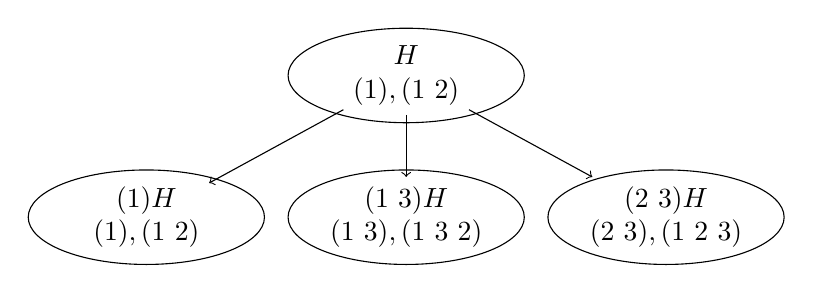
\begin{tikzpicture}[scale=0.6]
\draw (0, 3) circle[x radius=2.5cm, y radius=1cm] node[align=center] (H) {$H$ \\ $(1), (1\ 2)$}
      (-5.5, 0) circle[x radius=2.5cm, y radius=1cm] node[align=center] (H1) {$(1) H$ \\ $(1), (1\ 2)$}
      (0, 0) circle[x radius=2.5cm, y radius=1cm] node[align=center] (H13) {$(1\ 3) H$ \\ $(1\ 3), (1\ 3\ 2)$}
      (5.5, 0) circle[x radius=2.5cm, y radius=1cm] node[align=center] (H23) {$(2\ 3) H$ \\ $(2\ 3), (1\ 2\ 3)$};
\draw[->] (H) edge (H1)
          (H) edge (H13)
          (H) edge (H23);
\end{tikzpicture}
\end{figure*}

Multiply the subgroup $H = \{(1), (1\ 2)\}$ from left with (1), (1 3), and (2 3) gives:

\blre
(1) H & = & \{(1), (1\ 2)\} \\
(1\ 3) H & = & \{(1\ 3), (1\ 3\ 2)\} \\
(2\ 3) H & = & \{(2\ 3), (1\ 2\ 3)\} \\
\elre

\item {Today is Sunday, what day it will be after $2^{100}$ days?}

There are 7 days in a week. According to the Fermat's little theorem, $2^{7-1} \equiv 1 \mod 7$. We have:

\blre
2^{100} = 2^{16 \times 6 + 4} & \equiv & 1 \times 2^4 \mod 7 \\
  & \equiv & 16 \mod 7 \\
  & \equiv & 2 \mod 7 \\
\elre

Therefore, it will be Tuesday.

\item {Given two strings (character string or list), write a program to test if they form the same necklace.}

Given two strings $S_1, S_2$ with the same length, we can duplicate $S_1$ and append it after itself, then examine whether $S_2$ is the sub-string of $S_1S_1$. If yes, then they can form the same necklace.

\[
eqiv(S_1, S_2) = S_2 \subset (S_1 \doubleplus S_1)
\]

\lstset{language=Python, frame=single}
\begin{lstlisting}
def eqiv(s1, s2):
    return (s1 + s1).find(s2) != -1
\end{lstlisting}

\item {Write a program to realize Eratosthenes sieve algorithm.}

For all natural numbers from 2, pick the next as a prime, then remove all its multiplicands. Then do this repeatedly. Here is an example Haskell program:

\lstset{language=Haskell}
\begin{lstlisting}
primes = sieve [2..] where
    sieve (x:xs) = x : sieve [y | y <- xs, y `mod` x > 0]
\end{lstlisting}

The following are the example Python and Java programs.

\lstset{language=Python}
\begin{lstlisting}
def odds():
    i = 3
    while True:
        yield i
        i = i + 2

class prime_filter(object):
    def __init__(self, p):
        self.p = p
        self.curr = p

    def __call__(self, x):
        while x > self.curr:
            self.curr += self.p
        return self.curr != x

def sieve():
    yield 2
    iter = odds()
    while True:
        p = next(iter)
        yield p
        iter = filter(prime_filter(p), iter)

list(islice(sieve(), 100))
\end{lstlisting}

\lstset{language=Java}
\begin{lstlisting}
public class Prime {
    private static LongPredicate sieves = x -> true; // initialize sieve as id
    public final static long[] PRIMES = LongStream
        .iterate(2, i -> i + 1)
        .filter(i -> sieves.test(i))
        .peek(i -> sieves = sieves.and(v -> v % i != 0)) // update, chain the sieve
        .limit(100)                 // take first 100
        .toArray();
}
\end{lstlisting}

\item{Extend the idea of Eratosthenes sieve algorithm, write a program to generate Euler $\upphi$ function values for all numbers from 2 to 100.}

When generate prime numbers within $n$ with the sieve of Eratosthenes, we can update the Euler $\upphi$ function list by every prime numbers found so far. The function list is initialized with all element start from 1. For every prime number $p$, the corresponding $\upphi(p) = p(1 - \dfrac{1}{p}) = p - 1$. All the multiplicands of $p$ need multiply with this value. However, it is not enough as $\upphi(p^2) = p^2(1 - \dfrac{1}{p}) = p \upphi(p)$. Next we need multiply all the Euler function value for multiplicands of $p^2$ by $p$, and repeat for multiplicands of $p^3$ and so on until $p^m$ exceeds $n$. Below is the algorithm of this idea.

\begin{algorithmic}
\Function{Euler-Totient}{$n$}
  \State $\upphi \gets \{1, 1, ..., 1\}$ \Comment{1 to $n$}
  \State $P \gets \{2, 3, ..., n\}$ \Comment{sieve input}
  \While{$P \neq \varnothing$}
    \State $p \gets P[0]$
    \State $P \gets \{x | x \in P, x \bmod p \neq 0\}$
    \State $p' \gets p$
    \Repeat
      \For{$i \gets$ from $p'$ to $n$ step $p'$}
        \If{$p' = p$}
          \State $\upphi[i] \gets \upphi[i] \times (p - 1)$
        \Else
          \State $\upphi[i] \gets \upphi[i] \times p$
        \EndIf
      \EndFor
      \State $p' \gets p' \times p$
    \Until{$p' > n$}
  \EndWhile
  \State \Return $\upphi$
\EndFunction
\end{algorithmic}

\item {Write a program to realize fast modular multiplication, and Fermat's primality test.}

Our idea is to realize the fast modular multiplication with the similar approach when calculate power.

\[
x^y =
\begin{cases}
y \text{is even}: & x^{\lfloor y / 2 \rfloor} \\
y \text{is odd}: & x \cdot x^{\lfloor y / 2 \rfloor} \\
\end{cases}
\]

Based on this, we can change it to modular multiplication as below:

\begin{algorithmic}
\Function{Mod-Exp}{$x, y, n$}
  \If{$y = 0$}
    \State \Return 1
  \EndIf
  \State $z \gets$ \Call{Mod-Exp}{$x, \lfloor y /2 \rfloor, n$}
  \If{$y$是偶数}
    \State \Return $z^2 \bmod n$
  \Else
    \State \Return $x \cdot z^2 \bmod n$
  \EndIf
\EndFunction
\end{algorithmic}

With Fermat's little theorem, we can realize the primality test with some selected 'witnesses':

\begin{algorithmic}
\Function{primality}{$n$}
  \State random select $k$ positive numbers $a_1, a_2, ..., a_k < n$
  \If{$a_i^{n-1} \equiv 1 \mod n$, for all $i = 1, 2, ..., k$}
    \State \Return prime
  \Else
    \State \Return composite
  \EndIf
\EndFunction
\end{algorithmic}

\item {Prove the theorem that the two cancellation rules hold in a nonzero ring (ring without zero divisor).}

\begin{proof}
Suppose there is no zero divisor in $R$. Because
\[
  ab = ac \Rightarrow a(b - c) = 0
\]

as no zero divisor, hence:

\[
  a \neq 0, ab = ac \Rightarrow b - c = 0 \Rightarrow b = c
\]

Similarly,

\[
  a \neq 0, ba = ca \Rightarrow b = c
\]

Therefore, both cancellation rules hold in $R$. Reversely, suppose the first cancellation rule hold in $R$. Because:

\[
  ab = 0 \Rightarrow ab = a0
\]

Based on the assumption,

\[
  a \neq 0, ab = 0 \Rightarrow b = 0
\]

Hence $R$ does not have zero divisor. We can make the similar prove when the second cancellation rule holds.
\end{proof}

\item {Prove that, all real numbers in the form of $a + b \sqrt{2}$, where $a, b$ are integers form a integral domain under the normal addition and multiplication.}

\begin{proof}
We need verify three things:

  \begin{enumerate}[i]
  \item The commutative law for multiplication holds.
    \bre
      (a + b \sqrt{2})(c + d \sqrt{2}) & = & ac + 2bd + (ad + bc)\sqrt{2} \\
        & = & (c + d \sqrt{2})(a + b \sqrt{2})
    \ere
  \item There is unit 1 for multiplication.
    \[
      1 (a + b \sqrt{2}) = (a + b \sqrt{2}) 1 = a + b \sqrt{2}
    \]
  \item No zero divisor
    \[
    (a + b \sqrt{2})(c + d \sqrt{2}) = 0 \Rightarrow a = b = 0\ \text{or}\ c = d = 0
    \]
  \end{enumerate}
\end{proof}

\item {Prove that $Q[a, b] = Q[a][b]$, where $Q[a, b]$ contains all the expressions combined with $a$ and $b$, such as $2ab, a + a^2b$ etc.}

Let us see an example first:

\[
 Q[\sqrt{2}, \sqrt{3}] = \{a + b \sqrt{2} + c \sqrt{3} + d \sqrt{6}, \text{where} a, b, c, d \in Q\}
\]

\bre
Q[\sqrt{2}][\sqrt{3}] & = & \{a + b \sqrt{3}, \text{where} a, b \in Q[\sqrt{2}]\} \\
  & = & \{a' + b' \sqrt{2} + (c + d \sqrt{2}) \sqrt{3}, \text{where} a', b', c, d \in Q\} \\
  & = & \{a' + (b' + d) \sqrt{2} + c \sqrt{3} + d \sqrt{6}, \text{where} a', b', c, d \in Q\}
\ere

\begin{proof}
\[
Q[a][b] = \{x_0 + x_1 b + x_2 b^2 + ... + x_n b^n, \text{其中} x_i \in Q[a]\}
\]
$n$ is the minimum integer that polynomial $p(b) = 0$ exists. Substitute $x_i$ with the expressions in field $Q[a]$.

\bre
Q[a][b] & = & \{ y_{0,0} + y_{0,1} a + y_{0,2} a^2 + ... + y_{0,m} a^m + \\
        &   &   (y_{1,0} + y_{1,1} a + y_{1,2} a^2 + ... + y_{1,m} a^m) b + \\
        &   &   (y_{n,0} + y_{n,1} a + y_{n,2} a^2 + ... + y_{n,m} a^m) b^n \}
\ere

Where $y_{i,j} \in Q$, $m$ is the minimum integer that polynomial $p(a) = 0$ exists.

Without loss of generality, we assume $m < n$ (otherwise, we let $m' = min(m, n), n' = max(m, n)$). We can further convert it as:

\bre
Q[a][b] & = & \{ y_{0,0} + y_{0,1} a + y_{1,0} b + y_{0,2} a^2 + y_{1,1} ab + y_{2,0} b^2 + ... \\
        &   &    + y_{0,m} a^m + y_{1,m-1} a^{m-1} b + ... + y_{m, 0} b^m + \\
        &   &    + y_{1,m} a^m b + y_{2, m-1} a^{m-1} b^2 + ... + y_{m, 1} b^{m+1} + ... \\
        &   &    + y_{n, m} a^m b^n \}
\ere

This field is formed with all the expressions of $a, b$.
\end{proof}

\item {Prove that, for any polynomial $p(x)$, with rational coefficients, $E/Q$ is the field extension, $f$ is the $Q$-automorphism of $E$, then equation $f(p(x)) = p(f(x))$ holds.}

\begin{proof}
Because $f$ is automorphism, we have:

\[
f(x + y) = f(x) + f(y), f(ax) = f(a) f(x), f(1/x) = 1 / f(x)
\]

Further, since $f$ is $Q$-automorphism, we have:

\[
 f(x) = x, \forall x \in Q
\]

Let $p(x) = a_0 + a_1 x + ... + a_n x^n$, where $a_i \in Q$, then:

\bre
f(p(x)) & = & f(a_0 + a_1 x + ... + a_n x^n) \\
  & = & f(a_0) + f(a_1 x) + ... + f(a_n x^n) & f(x + y) = f(x) + f(y) \\
  & = & f(a_0) + f(a_1) f(x) + f(a_2) f(x)^2 + ... + f(a_n) f(x)^n & f(ax) = f(a) f(x) \\
  & = & a_0 + a_1 f(x) + a_2 f(x)^2 + ... + a_n f(x)^n & f(x) = x, \forall x \in Q \\
  & = & p(f(x)) \\
\ere
\end{proof}

\item{Taking the complex number into account, what is the splitting field for polynomial $p(x) = x^4-1$? What are the functions in its $Q$-automorphism?}

There are four roots for polynomial $x^4 -1$. They are $\pm 1, \pm i$. We can factor the polynomial to $p(x) = (x + 1)(x - 1)(x + i)( x - i)$. Actually, the splitting field of $p(x)$ is not complex number field $C$. It is too big. The splitting field is $Q[i]$.

There are two transformations in this $Q$-automorphism. One is $f(a + bi) = a - bi$, the other is the identity transformation $g(x) = x$.

\item{What's the Galois group for quadratic equation $x^2 - bx + c = 0$?}

We know the two roots for quadratic equation are:

\[
x_1, x_2 = \dfrac{b \pm \sqrt{b^2 - 4c}}{2}
\]

There are three cases: (1) there exists a rational number, such that $b^2 - 4c = r^2$. There are two rational roots (including duplicated ones) in this case; (2) No such rational number. Equation is not solvable in rational field, but there are real roots; (3) the discriminant is negative, hence the equation is not solvable in real field. But there are complex roots. Let's see the corresponding Galois groups for these three cases:

Case 1: there are two rational roots $\dfrac{b \pm r}{2}$. There is only one element in its Galois group, which is the identity automorphism $f(x) = x$.

Case 2: there are two irrational roots $\dfrac{b \pm \sqrt{d}}{2}$. There are two elements in its Galois group. One is the automorphism $f(p + q \sqrt{d}) = p - q \sqrt{d}$, where $p, q$ are rationals; the other is the identity transformation.

Case 3: There are two complex roots $\dfrac{b \pm i \sqrt{d}}{2}$. There are two elements in its Galois group. One is the automorphism $f(p + q i) = p - q i$, where $p, q$ are real numbers; the other is the identity transformation.

Actually, in case 2 and 3, their Galois groups are isomorphic in the splitting field. Note that $f(f(x)) = x$. It is isomorphic to the group of two elements ${0, 1}$ under the addition modulo 2. It is also isomorphic to the cyclic group $C_2$ or $\pmb{Z}/2\pmb{Z}$. Where the notation $\pmb{Z}/2\pmb{Z}$ means the quotation group of integers under addition $\pmb{Z}$ and its sub-group of even numbers $2\pmb{Z}$.

\item{Prove that, if $p$ is prime number, then Galois group for equation $x^p - 1$ is the ($p-1$)-cycle cyclic group $C_{p-1}$.}

The $p$ roots of $x^p - 1$ are the points along the unit circle in complex plane, i.e. $1, \omega, \omega^2, ..., \omega^{p-1}$. They can be expressed in form of $e^{2 \pi k i / p}$. The splitting field is $Q[\omega]$.

Consider automorphism $f$ as an element in Galois group $Gal(Q[\omega]/Q)$. According to the definition of automorphism, we have:

\[
f(\omega)^k = f(\omega^k) = 1 \iff \omega^k = 1
\]

It means $f(\omega)$ is also a $p$-th root of unity (a root of equation $x^p - 1 = 0$\footnote{If $p$ is not a prime number, but an integer $n$ greater than 1, then the $k$-th power of the $m$-th root can is $\zeta_m^k = e^{2 \pi m k i / n}$. There may exist some $k < n$, such that $\zeta_m^k = 1$. Actually, it holds as far as $n$ divides $mk$. However, if $n$ is a prime number $p$, then $k$ can't be less than $p$, but must be multiplicand of $p$.}). Denote:

\[
f(\omega) = h_i(\omega) = \omega^{i}
\]

If $f(\omega)$ is the $i$-th root of unity, we name it as $h_i$, where $1 \leq i \leq p-1$ (why $i$ can't be 0?). In this way, we establish a one-to-one mapping from Galois group to cyclic group $C_{p-1}$:

\[
Gal(Q[\omega]/Q) \arrowto{\sigma} C_{p-1} :  \sigma(h_i) = i
\]

Where the Galois group contains $p-1$ automorphisms $\{h_1, h_2, ..., h_{p-1}\}$, hence it has the same order as the cyclic group $C_{p-1}$.

Next we prove this is a group isomorphism.

\[
(h_i \cdot h_j)(\omega) = h_i(h_j(\omega)) = h_i(\omega^j) = \omega^{ji} = \omega^{ij}
\]

hence

\[
\sigma(h_i \cdot h_j) = ij = \sigma(h_i) \cdot \sigma(h_j)
\]

And $h_1(\omega)$ is the generator of this cyclic Galois group.

\begin{mdframed}
Here are two different groups that often cause confusion. The first one is the group of integers under addition modulo $n$. It's a cyclic group, containing the residue class modulo $n$ of \{ 0, 1, 2, ..., $n - 1$\}, total $n$ elements. This group is often denoted as $\pmb{Z}/n\pmb{Z}$. It is isomorphic to the group formed with the $n$ roots of equation $x^n - 1 = 0$. The elements are the $n$-th root of unity $\{1 = \zeta_n^0, \zeta_n^1, \zeta_n^2, ..., \zeta_n^{n-1}\}$. The binary operation is multiplication.

\vspace{5mm}

The second group is integers under multiplication modulo $n$. The group elements are not all the residues from 0 to $n-1$, but all the ones coprime to $n$. The group operation is modulo multiplication. Denoted as $(\pmb{Z}/n\pmb{Z})^{\times}$. There are total $\upphi(n)$ elements, where $\upphi$ is Euler's totient function. When $n$ is prime $p$, there are $\{1, 2, ..., p-1\}$, total $p-1$ group elements. However, the multiplicative group modulo $n$ is not necessary cyclic. Luckily it is cyclic when $n$ is prime. An interesting fact is that $(\pmb{Z}/p\pmb{Z})^{\times}$ is isomorphic to the additive group $\pmb{Z}/(p-1)\pmb{Z}$.

\vspace{5mm}

This exercise tells us: For the Galois group in rational field extension, if it is generated by $n$-th root of unity, then this group is isomorphic to the multiplicative group of integers modulo $n$, i.e. $(\pmb{Z}/n\pmb{Z})^{\times}$. For example, the cubic equation $x^3 -1 = 0$ has three roots $\{1, \dfrac{-1 \pm i \sqrt{3}}{2}\}$. Its Galois group contains two automorphisms. One is $f(x) = x$, which is corresponding to $h_1(\omega) = \omega^1$; the other is $g(a + bi) = a - bi$, which is corresponding to $h_2(\omega) = \omega^2$. The effect of $h_2$ is transform the order of the three roots from $1, 2, 3$ to $1, 3, 2$.

\[
\begin{array}{l}
1 \mapsto 1^2 = 1 \\
\omega \mapsto \omega^2 \\
\omega^2 \mapsto (\omega^2)^2 = \omega^3 \omega = \omega \\
\end{array}
\]

\end{mdframed}

\item {The 5th degree equation $x^5 - 1 = 0$ is radical solvable. What's its Galois subgroup chain?}

From previous exercise, we know the 5 roots are points along the unit circle in the complex plane: \{1, $\zeta$, $\zeta^2$, $\zeta^3$, $\zeta^4$ \}, where $\zeta = e^{2 \pi i / 5} = \dfrac{\sqrt{5} - 1 + \sqrt{10 + 2 \sqrt{5}}}{4}$. The Galois group in rational field is a cyclic group of order 4: $G(Q[\zeta]/Q) = C_4$. It is isomorphic to the multiplicative group modulo 5: $(\pmb{Z}/5\pmb{Z})^{\times} = \{1, 2, 3, 4 \}_5$. There is no intermediate field extension. The splitting field is $Q[\zeta]$. The Galois group in splitting field is $\{1\}$.

Obviously, $\{1\}$ is the normal subgroup of $C_4$. The quotient group $C_4/\{1\}$ is cyclic too. In previous exercise, we proved that cyclic group is abelian, hence the equation is radical solvable.

\end{enumerate}

\section{categories}

\begin{enumerate}
\item {Prove that the identity arrow is unique (hint: refer to the uniqueness of identity element for groups in the previous chapter).}

Suppose there exists another identity arrow $id_A'$, pointed $A$ from itself: $A \arrowto{id_A'} A$.

Consider every arrow from $A$ to $B$: $A \arrowto{f} B$, from the definition of identity arrow, $f \circ id_A = f$ holds. When replace $B$ with $A$, and replace $f$ with $id_A'$, then:

\[
id_A' \circ id_A = id_A'
\]

Similar, from every arrow from $B$ to $A$: $B \arrowto{g} A$, from the definition of identity arrow, $id_A' \circ g = g$ holds. When replace $B$ with $A$, replace $g$ with $id_A$, then:

\[
id_A' \circ id_A = id_A
\]

Summarize these two result, we obtain $id_A = id_A'$, hence the identity arrow is unique.

\item {Verify the monoid $(S, \cup, \varnothing)$ (the elements are sets, the binary operation is set union, the identity element is empty set) and $(N, +, 0)$ (elements are natural numbers, the binary operation is add, the identity element is zero) are all categories that contain only one object.}

The key idea is that every monoid is a category contains only one object. It's a bit difficult to answer: what is the object in this category? In fact, it does not matter what this object is. The object is not necessary the monoid, or any given set. It even need not contain any elements. To avoid bother with concrete object, we give it notation $\bigstar$.

Let's first see the set monoid under union. Every set as an element in the monoid $s \in S$ can be used to define an arrow:

\[
\bigstar \arrowto{s} \bigstar
\]

Note there is no any inner structure (of the monoid) involved. The arrow composition is exactly set union.

\begin{center}
\begin{tikzpicture}
  \matrix (m) [matrix of math nodes,
               row sep=3em, column sep=4em, minimum width=2em]{
     & \bigstar & \\
     \bigstar & & \bigstar \\};
  \path[-stealth]
    (m-2-1) edge node [above] {$s_1$} (m-1-2)
    (m-1-2) edge node [above] {$s_2$} (m-2-3)
    (m-2-1) edge node [below] {$s_1 \circ s_2 = s_1 \cup s_2$} (m-2-3);
\end{tikzpicture}
\end{center}

Because set union is associative, the arrows is also associative. The empty set is the unit of this monoid, it defines the identity arrow. As the empty set union any set equals to that set itself, it serves as the identity arrow. Such that the set monoid under union do form a category contains only one object.

\begin{figure}[htbp]
\centering
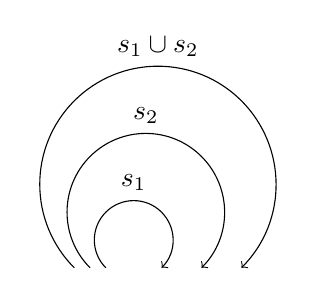
\begin{tikzpicture}
\path (0, 0) node (obj) {$\bigstar$};
\draw[->] (-0.2, 0) arc[radius=5mm, start angle=225, end angle=-45] node[pos=0.5, above]{$s_1$};
\draw[->] (-0.4, 0) arc[radius=10mm, start angle=225, end angle=-45] node[pos=0.5, above]{$s_2$};
\draw[->] (-0.6, 0) arc[radius=15mm, start angle=225, end angle=-45] node[pos=0.5, above]{$s_1 \cup s_2$};
\end{tikzpicture}
\captionsetup{labelformat=empty}
\end{figure}

Next let us see the additive monoid for natural numbers. Every number $n$ can define an arrow:

\[
\bigstar \arrowto{n} \bigstar
\]

The arrow composition is addition. Since addition is associative, hence arrow composition is also associative. Zero, 0 defines the identity arrow. This is because 0 add to any number equals to this number itself. Therefore, the additive monoid for natural numbers do form a category.

\begin{figure}[htbp]
\centering
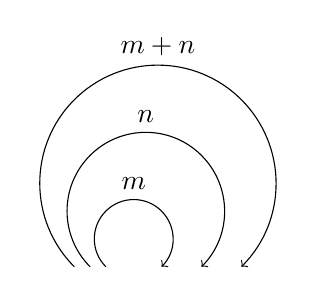
\begin{tikzpicture}
\path (0, 0) node (obj) {$\bigstar$};
\draw[->] (-0.2, 0) arc[radius=5mm, start angle=225, end angle=-45] node[pos=0.5, above]{$m$};
\draw[->] (-0.4, 0) arc[radius=10mm, start angle=225, end angle=-45] node[pos=0.5, above]{$n$};
\draw[->] (-0.6, 0) arc[radius=15mm, start angle=225, end angle=-45] node[pos=0.5, above]{$m + n$};
\end{tikzpicture}
\captionsetup{labelformat=empty}
\end{figure}


\item {In chapter 1, we introduced Peano's axioms for natural numbers as well as the isomorphic structures to Peano arithmetic, like the linked-list etc. They can be described in categories. This was found by German mathematician Richard Dedekind although the category theory was not established by his time. We named this category as Peano category, denoted as $\pmb{Pno}$. The objects in this category is $(A, f, z)$, where $A$ is a set, for example natural numbers $N$; $f: A \to A$ is a successor function. It is $succ$ for natural numbers; $z \in A$ is the starting element, it is zero for natural numbers. Given any two Peano objects $(A, f, z)$ and $(B, g, c)$, define the morphism from $A$ to $B$ as:

\[
A \arrowto{\phi} B
\]

It satisfies:

\[
\phi \circ f = g \circ \phi \quad \text{and} \quad \phi(z) = c
\]

Verify that $\pmb{Pno}$ is a category.}

An object in Peano category is a tuple of $(A, f, z)$. An arrow is a map $\phi$ that preserve the tuple structure. Arrow composition is function composition:

\[ \begin{array}{l}
A \arrowto{\phi} B \arrowto{\psi} C \\
A \arrowto{\psi \circ \phi} C
\end{array}\]

Because function composition is associative, hence arrow composition is associative. For identity arrow:

\[
A \arrowto{id_A} A
\]

It satisfies $id_A(z) = z$, and $id_A \circ f = f \circ id_A$.

Obviously, the tuple $(\pmb{N}, succ, 0)$ is an object in Peano category. It's interesting that, for every object $(A, f, z)$ in Peano category, there is a unique arrow:

\[
(\pmb{N}, succ, 0) \arrowto{\sigma} (A, f, z)
\]

where:

\[
\sigma(n) = f^n(z)
\]

which maps any natural number $n$ to the result of applying $f$ to $z$ for $n$ times.

\item {请使用叠加操作$foldr$来定义列表函子的箭头映射。}

本质上就是用$foldr$定义列表的逐一映射:

\[
fmap\ f = foldr\ f\ Nil
\]

\item {证明可能函子和列表函子的组合$\mathbf{Maybe} \circ \mathbf{List}$与$\mathbf{List} \circ \mathbf{Maybe}$仍然是函子。}

我们只证明$\mathbf{Maybe} \circ \mathbf{List}$仍然是函子。另一证明与此类似。任何对象$A$被映射为$\mathbf{Maybe} (\mathbf{List}\ A)$。对于箭头,我们先看恒等箭头的情况:

\bre
(\mathbf{Maybe} \circ \mathbf{List})\ id & = & \mathbf{Maybe} (\mathbf{List}\ id) & \text{函子的组合} \\
 & = & \mathbf{Maybe}\ id & \text{列表函子的恒等箭头} \\
 & = & id & \text{可能函子的恒等箭头} \\
\ere

然后是箭头组合:

\bre
(\mathbf{Maybe} \circ \mathbf{List})\ (f \circ g) & = & \mathbf{Maybe} (\mathbf{List}\ (f \circ g)) & \text{函子的组合} \\
 & = & \mathbf{Maybe} ((\mathbf{List}\ f) \circ (\mathbf{List}\ g)) & \text{列表函子的箭头组合性质} \\
 & = & (\mathbf{Maybe}\ (\mathbf{List}\ f)) \circ (\mathbf{Maybe}\ (\mathbf{List}\ g)) & \text{可能函子的箭头组合性质} \\
 & = & ((\mathbf{Maybe} \circ \mathbf{List})\ f) \circ ((\mathbf{Maybe} \circ \mathbf{List})\ g) & \text{函子的组合} \\
\ere

\item {证明任意函子的组合$\mathbf{G} \circ \mathbf{F}$仍然是函子。}

仿照前一题,我们分别函子的组合满足恒等箭头,和箭头组合的性质即可。首先是恒等箭头性质:

\bre
(\mathbf{G} \circ \mathbf{F})\ id & = & \mathbf{G} (\mathbf{F}\ id) & \text{函子的组合} \\
 & = & \mathbf{Maybe}\ id & \text{函子$\mathbf{F}$的恒等箭头} \\
 & = & id & \text{函子$\mathbf{G}$的恒等箭头} \\
\ere

然后是箭头组合:

\bre
(\mathbf{G} \circ \mathbf{F})\ (\phi \circ \psi) & = & \mathbf{G} (\mathbf{F}\ (\phi \circ \psi)) & \text{函子的组合} \\
 & = & \mathbf{G} ((\mathbf{F}\ \phi) \circ (\mathbf{F}\ \psi)) & \text{函子$\mathbf{F}$的箭头组合性质} \\
 & = & (\mathbf{G}\ (\mathbf{F}\ \phi)) \circ (\mathbf{G}\ (\mathbf{F}\ \psi)) & \text{函子$\mathbf{G}$的箭头组合性质} \\
 & = & ((\mathbf{G} \circ \mathbf{F})\ \phi) \circ ((\mathbf{G} \circ \mathbf{F})\ \psi) & \text{函子的组合} \\
\ere

\item {思考一个预序集范畴上的函子的例子。}

预序集范畴上的函子是一个单调映射。
% monotone function(map)

\item {回顾第二章中介绍的二叉树,请定义一个二叉树函子。}

考虑集合全函数范畴上的对象$A$,二叉树函子将其映射为:

\lstset{language=Haskell, frame=none}
\begin{lstlisting}
data Tree A = Empty | Branch (Tree A) A (Tree A)
\end{lstlisting}

对于箭头$A \arrowto{f} B$,二叉树函子将其映射为:

\bre
fmap\ f\ Empty & = & Empty \\
fmap\ f\ (Branch\ l\ x\ r) & = & Branch\ (fmap\ f\ l)\ (f\ x)\ (fmap\ f\ r) \\
\ere

或者利用第二章定义的$mapt$:

\[
fmap = mapt
\]

\item {考虑偏序集(poset)中的两个对象,它们的积是什么?余积是什么?}

第三章中,我们说到一个偏序集本身就是一个范畴,每个元素都是一个对象,任何两个对象间最多有一个箭头(如果有序关系,则存在箭头)。对于偏序集中的两个元素(对象)$a$和$b$,如果它们都有指向上下游的箭头,则

\[
\text{交运算meet}\ a \land b \quad \quad \quad \text{并运算join}\ a \lor b
\]

是这一对对象的

\[
\text{积} \quad \quad \quad \text{余积}
\]

其中交运算是两个对象的最小上界,而并运算是两个对象的最大下界。由于最小上界和最大下界并不一定存在,所以偏序集中任何两个对象的积和余积也并不一定存在。

% https://en.wikipedia.org/wiki/Join_and_meet
%In mathematics, specifically order theory, the join and meet of a subset S of a partially ordered set P are respectively the supremum (least upper bound) of S, denoted ⋁S, and infimum (greatest lower bound) of S, denoted ⋀S. In general, the join and meet of a subset of a partially ordered set need not exist. Join and meet are dual to one another with respect to order inversion.

%\item {考虑集合范畴$\pmb{Set}$,积中的两个箭头$fst, snd$是右消去(epic)的么?余积中的两个箭头$left, right$是左消去(monic)的么?}
\item {证明余积的吸收率,并验证余积函子的组合性质。}

余积的吸收率是:

\[
[p, q] \circ (f + g) = [p \circ f, q \circ g]
\]

\begin{proof}
\blre
  & [p, q] \circ (f + g)  \\
= & [p, q] \circ [left \circ f, right \circ g] & \text{$+$的定义} \\
= & [[p, q] \circ (left \circ f), [p, q] \circ (right \circ g)] & \text{余积的融合律} \\
= & [[p, q] \circ left \circ f, [p, q] \circ right \circ g] & \text{结合性} \\
= & [p \circ f, q \circ g] & \text{余积的消去律} \\
\elre
\end{proof}

余积函子的组合性质:

\[
 (f + g) \circ (f' + g') = f \circ f' + g \circ g'
\]

\begin{proof}
令$p = left \circ f$,$q = right \circ g$

\blre
  & (f + g) \circ (f' + g') \\
= & [left \circ f, right \circ g] \circ (f' + g') & \text{$+$的定义} \\
= & [p, q] \circ (f' + g') & \text{用$p, q$代换} \\
= & [p \circ f', q \circ g'] & \text{余积的吸收律} \\
= & [left \circ f \circ f', right \circ g \circ g'] & \text{把$p, q$代回} \\
= & [left \circ (f \circ f'), right \circ (g \circ g')] & \text{结合律} \\
= & f \circ f' + g \circ g' & \text{反向用$+$的定义} \\
\elre
\end{proof}

\item {证明$swap$满足自然变换的条件$(g \times f) \circ swap = swap \circ (f \times g)$}

对于$A \arrowto{f} C$和$B \arrowto{g} D$,我们要证明下面的范畴图可交换。

\begin{center}
\begin{tikzpicture}
  \matrix (m) [matrix of math nodes,
               row sep=3em, column sep=5em, minimum width=2em]{
     (A, B) & (B, A) \\
     (C, D) & (D, C) \\};
  \path[-stealth]
    (m-1-1) edge node [above] {$swap_{A, B}$} (m-1-2)
    (m-2-1) edge node [below] {$swap_{C, D}$} (m-2-2)
    (m-1-1) edge node [left] {$f \times g$} (m-2-1)
    (m-1-2) edge node [right] {$g \times f = swap\ f \times g$} (m-2-2);
\end{tikzpicture}
\end{center}

\begin{proof}
\blre
  & ((g \times f) \circ swap)\ (A, B) \\
= & (g \times f)\ (swap\ (A, B)) & \text{组合的定义} \\
= & (g \times f) \circ (B, A) & \text{$swap$的定义} \\
= & (g\ B, f\ A) & \text{箭头的积} \\
= & (D, C) & \text{箭头$g, f$的定义} \\
= & swap\ (C, D) & \text{反向用$swap$的定义} \\
= & swap\ (f\ A, g\ B) & \text{反向用$f, g$的定义} \\
= & swap\ ((f \times g)\ (A, B)) & \text{箭头的积} \\
= & (swap \circ (f \times g))\ (A, B) & \text{反向用组合的定义} \\
\elre
\end{proof}

\item {证明多态函数$length$是一个自然变换,其定义如下:
\[
\begin{array}{l}
length : [A] \to Int \\
length\ [] = 0 \\
length\ (x:xs) = 1 + length\ xs
\end{array}
\]
}

对于任何对象$A$,它的索引箭头$length$为:

\[
[A] \arrowto{length_A} \mathbf{K}_{Int}\ A
\]

其中$\mathbf{K}_{Int}$是常函子,它将任何对象映射到$Int$,所有箭头映射为恒等箭头$id_{int}$。对于箭头$A \arrowto{f} B$,我们要证明下面的范畴图可交换。

\begin{center}
\begin{tikzpicture}
  \matrix (m) [matrix of math nodes,
               row sep=3em, column sep=5em, minimum width=2em]{
     A & \lbrack A \rbrack & \mathbf{K}_{Int}\ A \\
     B & \lbrack B \rbrack & \mathbf{K}_{Int}\ B \\};
  \path[-stealth]
    (m-1-1) edge node [left] {$f$} (m-2-1)
    % square
    (m-1-2) edge node [above] {$length_A$} (m-1-3)
    (m-2-2) edge node [below] {$length_B$} (m-2-3)
    (m-1-2) edge node [left] {$\mathbf{List}(f)$} (m-2-2)
    (m-1-3) edge node [right] {$\mathbf{K}_{Int}(f)$} (m-2-3);
\end{tikzpicture}
\end{center}

利用常函子的定义,这个范畴图等价于:

\begin{center}
\begin{tikzpicture}
  \matrix (m) [matrix of math nodes,
               row sep=3em, column sep=5em, minimum width=2em]{
     A & \lbrack A \rbrack & Int \\
     B & \lbrack B \rbrack & Int \\};
  \path[-stealth]
    (m-1-1) edge node [left] {$f$} (m-2-1)
    % square
    (m-1-2) edge node [above] {$length_A$} (m-1-3)
    (m-2-2) edge node [below] {$length_B$} (m-2-3)
    (m-1-2) edge node [left] {$\mathbf{List}(f)$} (m-2-2)
    (m-1-3) edge node [right] {$id$} (m-2-3);
\end{tikzpicture}
\end{center}

也就是要证明:

\[
id \circ length_{A} = length_{B} \circ \mathbf{List}(f)
\]

即:$length_{A} = length_{B} \circ \mathbf{List}(f)$


\begin{proof}
我们用数学归纳法证明。首先是空列表:

\blre
  & length_B \circ \mathbf{List}(f) [] \\
= & length_B [] & \text{列表函子的定义} \\
= & 0 & \text{$length$的定义} \\
= & length_A\ [] & \text{反向用$length$的定义}
\elre

然后是归纳假设,设$length_B \circ \mathbf{List}(f)\ as = length_A\ as$成立,我们有:

\blre
  & length_B \circ \mathbf{List}(f) (a:as) \\
= & length_B\ (f(a) : \mathbf{List}(f)\ as) & \text{列表函子的定义} \\
= & 1 + length_B\ (\mathbf{List}(f)\ as) & \text{$length$的定义} \\
= & 1 + length_B\ \circ \mathbf{List}(f)\ as & \text{箭头组合} \\
= & 1 + length_A\ as & \text{归纳假设} \\
= & length_A\ (a:as) & \text{反向用$length$的定义}
\elre
\end{proof}

\item {自然变换也可以进行组合,考虑两个自然变换$\mathbf{F} \arrowto{\phi} \mathbf{G}$和$\mathbf{G} \arrowto{\psi} \mathbf{H}$,对于任意箭头$A \arrowto{f} B$,试画出自然变换组合$\phi \circ \psi$的范畴图,并列出可交换性的条件。}

\begin{center}
\begin{tikzpicture}
  \matrix (m) [matrix of math nodes,
               row sep=3em, column sep=5em, minimum width=2em]{
     \mathbf{F}A & \mathbf{G}A & \mathbf{H}A \\
     \mathbf{F}B & \mathbf{G}B & \mathbf{H}B \\};
  \path[-stealth]
    (m-1-1) edge node [left] {$\mathbf{F}(f)$} (m-2-1)
    (m-1-1) edge node [above] {$\phi_A$} (m-1-2)
    (m-2-1) edge node [below] {$\phi_B$} (m-2-2)
    (m-1-2) edge node [above] {$\psi_A$} (m-1-3)
    (m-2-2) edge node [below] {$\psi_B$} (m-2-3)
    (m-1-2) edge node [left] {$\mathbf{G}(f)$} (m-2-2)
    (m-1-3) edge node [right] {$\mathbf{H}(f)$} (m-2-3);
\end{tikzpicture}
\end{center}

可交换的条件为:

\[
\mathbf{H}(f) \circ (\psi_A \circ \phi_A) = (\psi_B \circ \phi_B) \circ \mathbf{F} (f)
\]

\item{在本节的例子中,我们说在一个偏序集中,如果存在最小值(或最大值),则最小值(或最大值)就是起始对象(或终止对象)。考虑全体偏序集构成的范畴$\pmb{Poset}$,如果存在起始对象,它是什么?如果存在终止对象,它是什么?}

对于$\pmb{Poset}$范畴,对象是偏序集,箭头是单调映射。对于两个偏序集$P, Q$,箭头$P \arrowto{h} Q$使得偏序集$P$中任何两个有序元素$a \leq b$,有$h(a) \leq h(b)$。

这一范畴中的起始对象是空偏序集$0 = \varnothing$。它到任何其它偏序集有唯一的箭头:

\[
\varnothing \longrightarrow P
\]

终止对象是之后一个元素的偏序集$1 = \{\bigstar\}$,偏序关系为$R = \{(\bigstar, \bigstar)\}$,即$\bigstar \leq \bigstar$。任何偏序集$P$到1有唯一的箭头:

\bre
P & \longrightarrow & \{\bigstar\} \\
p & \mapsto & \bigstar
\ere

\item{皮亚诺范畴$\pmb{Pno}$(参见本章第一节的习题2)中,什么样的对象$(A, f, z)$是起始对象?终止对象是什么?}

起始对象是$(\pmb{N}, succ, 0)$,它到任何其它对象唯一箭头是:

\[
(\pmb{N}, succ, 0) \arrowto{\sigma} (A, f, z): \sigma(n) = f^n(z)
\]

终止对象是只有一个元素的对象$1 = (\{\bigstar\}, \bigstar, id)$。任何皮亚诺范畴的对象$(A, f, z)$到终止对象的唯一箭头是:

\[
(A, f, z) \arrowto{\sigma} 1 : \sigma(a) = \bigstar
\]

\item{验证$\pmb{Exp}$的确是一个范畴,指出$id$箭头和箭头的组合。}

我们先看$id$箭头的定义$h \arrowto{id} h$,它使得下面的范畴图可交换:

\begin{center}
\begin{tikzpicture}
  \matrix (m) [matrix of math nodes,
               row sep=3em, column sep=5em, minimum width=2em]{
     A & A \times B & \\
     A & A \times B & C \\};
  \path[-stealth]
    (m-1-1) edge node [left] {$id_A$} (m-2-1)
    (m-1-2) edge node [left] {$id_A \times id_B$} (m-2-2)
    (m-1-2) edge node [above] {$h$} (m-2-3)
    (m-2-2) edge node [below] {$h$} (m-2-3);
\end{tikzpicture}
\end{center}

然后是箭头组合:

$h \arrowto{i} k$和$k \arrowto{j} m$的组合是$j \circ i$使得下面的范畴图交换:

\begin{center}
\begin{tikzpicture}
  \matrix (m) [matrix of math nodes,
               row sep=3em, column sep=5em, minimum width=2em]{
     A & A \times B & \\
     D & D \times B & C \\
     E & E \times B & \\};
  \path[-stealth]
    (m-1-1) edge node [left] {$f$} (m-2-1)
    (m-2-1) edge node [left] {$g$} (m-3-1)
    (m-1-2) edge node [left] {$f \times id_B$} (m-2-2)
    (m-2-2) edge node [left] {$g \times id_B$} (m-3-2)
    (m-1-2) edge node [above] {$h$} (m-2-3)
    (m-2-2) edge node [above] {$k$} (m-2-3)
    (m-3-2) edge node [below] {$m$} (m-2-3);
\end{tikzpicture}
\end{center}

因此对于箭头$h \arrowto{j} k$有:$id_k \circ j = j = j \circ id_h$。并且对于三个箭头有结合律。

\item{反射律$curry\ apply = id$中,$id$的下标是什么?请用另一种方法证明它。}

$id$的下标是二元箭头的类型$A \times B \to C$。

\begin{proof}
\blre
  & curry \circ apply\ f\ a\ b \\
= & curry\ (apply\ f)\ a\ b & \text{组合的定义} \\
= & (apply\ f)\ (a, b) & \text{$curry$的定义}\\
= & f(a, b) & \text{$apply$的定义} \\
= & id_{A \times B \to C}\ f(a, b)
\elre
\end{proof}

\item{我们称下面的等式
\[
(curry\ f) \circ g = curry(f \circ (g \times id))
\]
为克里化的融合律。请画出它的范畴图并证明它。}

\begin{center}
\begin{tikzpicture}
  \matrix (m) [matrix of math nodes,
               row sep=3em, column sep=5em, minimum width=2em]{
     D & D \times B & \\
     A & A \times B & \\
     C^B & C^B \times B & C \\};
  \path[-stealth]
    (m-1-1) edge node [left] {$g$} (m-2-1)
    (m-2-1) edge node [left] {$curry\ f$} (m-3-1)
    (m-1-2) edge node [left] {$g \times id$} (m-2-2)
    (m-1-2) edge [bend right] node {} (m-3-2)
    (m-1-2) edge node [above] {$f \circ (g \times id)$} (m-3-3)
    (m-2-2) edge node [above] {$f$} (m-3-3)
    (m-3-2) edge node [below] {$apply$} (m-3-3);
\end{tikzpicture}
\end{center}

观察图中$D \times B$,$A \times B$,和$C$这个三角形。我们知道$D \times B \to A$这个组合箭头为$f \circ (g \times id)$。

根据幂对象和转换箭头的定义有:

\[
apply \circ (curry f) \circ g = f \circ (g \times id)
\]

由$curry$和$apply$的泛性性质有:

\[
(curry f) \circ g = curry (f \circ (g \times id)
\]

\item{画出群的可逆性公理的范畴图。}

可逆性公里表示为:$m \circ (id, i) = m \circ (i, id) = e$

\begin{center}
\begin{tikzpicture}
  \matrix (m) [matrix of math nodes,
               row sep=3em, column sep=5em, minimum width=2em]{
     G & G \times G & G \\
     1 & G & 1 \\};
  \path[-stealth]
    (m-1-1) edge node [above] {$(id, i)$} (m-1-2)
    (m-1-3) edge node [above] {$(i, id)$} (m-1-2)
    (m-1-1) edge node [left] {} (m-2-1)
    (m-1-2) edge node [left] {$m$} (m-2-2)
    (m-1-3) edge node [left] {} (m-2-3)
    (m-2-1) edge node [above] {$e$} (m-2-2)
    (m-2-3) edge node [above] {$e$} (m-2-2);
\end{tikzpicture}
\end{center}

\item{$p$是一个素数,使用群的F-代数,为整数模$p$乘法群(可以参考上一章)定义一个$\alpha$箭头。}

根据群的$\alpha$箭头定义:

\[
\mathbf{F} A \arrowto{\alpha = e + m +i} A
\]
定义整数模$p$乘法群如下:

\bre
e\ () & = & 1 & \text{单位元是1} \\
m(a, b) & = & ab \bmod p & \text{二元运算是模$p$乘法} \\
i(a) & = & a^{p-2} \bmod p & \text{根据费马小定理$a^{p-1} \equiv 1 \mod p$} \\
\ere

\item{参考上一章环的定义,定义环的F-代数。}

环上的代数结构由三部分组成:
\begin{enumerate}[i]
\item 携带对象$R$,用于携带环上代数结构的集合。
\item 多项式函子$\mathbf{F}A = 1 + 1 + A \times A + A \times A + A$。
\item 箭头$\mathbf{F}A \arrowto{\alpha = z + e + p + m + n} A$,它们分别是加法单位元$z$,乘法单位元$e$,加法$p$,乘法$m$,和求反$n$。
\end{enumerate}
这样就定义了一个环上的$F$-代数$(R, \alpha)$。例如当携带对象是整数时,算术运算下的环定义为:

\[\begin{array}{l}
z\ () = 0 \\
e\ () = 1 \\
p(a, b) = a + b \\
m(a, b) = ab \\
n(a) = -a \\
\end{array}\]

\item{F-代数范畴上的$id$箭头是什么?箭头组合是什么?}

从$F$-代数$(A, \alpha)$到其自身的同态映射是$id$箭头。箭头组合是$F$-态射的组合。携带对象间的箭头:$A \arrowto{f} B \arrowto{g} C$使得下面的范畴图可交换:

\begin{center}
\begin{tikzpicture}
  \matrix (m) [matrix of math nodes,
               row sep=3em, column sep=5em, minimum width=2em]{
     \mathbf{F} A & \mathbf{F} B & \mathbf{F} C \\
     A & B & C \\};
  \path[-stealth]
    (m-1-1) edge node [left] {$\alpha$} (m-2-1)
    (m-1-2) edge node [left] {$\beta$} (m-2-2)
    (m-1-3) edge node [left] {$\gamma$} (m-2-3)
    (m-1-1) edge node [above] {$\mathbf{F}(f)$} (m-1-2)
    (m-1-2) edge node [above] {$\mathbf{F}(g)$} (m-1-3)
    (m-2-1) edge node [below] {$f$} (m-2-2)
    (m-2-2) edge node [below] {$g$} (m-2-3);
\end{tikzpicture}
\end{center}

\[
  g \circ f \circ \alpha = \gamma \circ \mathbf{F}(g) \circ \mathbf{F}(f) = \gamma \circ \mathbf{F}(g \circ f)
\]

\item{可否把类自然数函子写成如下递归的形式?谈谈你的看法。
\begin{lstlisting}
data NatF A = ZeroF | SuccF (NatF A)
\end{lstlisting}
}

不可以。考虑携带对象$A$,上述函子$\mathbf{NatF}$是迭代的,它并不将$A$映射为确定的某个对象。事实上,我们希望把它映射为皮亚诺范畴上的对象$(A, z, f)$。

\item{我们可以为$\mathbf{NatF} Int \to Int$定义一个$\alpha$箭头,名叫$eval$:
\[
\begin{array}{l}
eval : \mathbf{NatF} Int \to Int \\
eval\ ZeroF = 0 \\
eval\ (SuccF\ n) = n + 1 \\
\end{array}
\]
如果迭代地将$A' = \mathbf{NatF} A$代入$\mathbf{NatF}$函子$n$次。我们把这样得到的函子记为$\mathbf{NatF}^n A$。试思考能否定义下面的$\alpha$箭头:
\[
\begin{array}{l}
eval : \mathbf{NatF}^n Int \to Int \\
\end{array}
\]
}

\bre
eval & : &\mathbf{NatF}^n Int \to Int \\
eval\ ZeroF & = & 0 & \text{$ZeroF$是$\mathbf{NatF}^n Int$的对象}\\
eval\ (SuccF\ ZeroF) & = & 1 & \text{$ZeroF$是$\mathbf{NatF}^{n-1} Int$的对象}\\
eval\ (SuccF\ (SuccF\ ZeroF)) & = & 2 & \text{$ZeroF$是$\mathbf{NatF}^{n-2} Int$的对象}\\
... \\
eval\ (SuccF^{n-1}\ ZeroF) & = & n - 1 & \text{$ZeroF$是$\mathbf{NatF} Int$的对象}\\
eval\ (SuccF^n\ m) & = & m + n \\
\ere

\item{对二叉树函子$\mathbf{TreeF}\ A\ B$,固定$A$,利用不动点验证$(\mathbf{Tree}\ A, [nil, branch])$是初始代数。}

令$B' = \mathbf{TreeF}\ A\ B$,然后不断递归地应用到自己,把此结果称为$\mathbf{Fix}\ (\mathbf{TreeF}\ A)$。

\bre
\mathbf{Fix}\ (\mathbf{TreeF}\ A) & = & \mathbf{TreeF}\ A\ (\mathbf{Fix}\ (\mathbf{TreeF}\ A)) & \text{不动点的定义} \\
 & = & \mathbf{TreeF}\ A\ (\mathbf{TreeF}\ A (...)) & \text{递归展开} \\
 & = & NilF | BrF\ A\ (\mathbf{TreeF}\ A\ (...))\ (\mathbf{TreeF}\ A\ (...)) & \text{二叉树函子的定义} \\
 & = & NilF | BrF\ A\ (\mathbf{Fix}\ (\mathbf{TreeF}\ A))\ (\mathbf{Fix}\ (\mathbf{TreeF}\ A)) & \text{反向用不动点} \\
\ere

比较$Tree A$的定义:

\begin{lstlisting}
data Tree A = Nil | Br A (Tree A) (Tree A)
\end{lstlisting}

故而:$\mathbf{Tree}\ A = \mathbf{Fix}\ (\mathbf{TreeF}\ A)$。初始代数为$(\mathbf{Tree}\ A, [nil, branch])$。

\end{enumerate}

\section{融合}

\begin{enumerate}
\item {验证从左侧叠加也可以表示为$foldr$:
\[
foldl\ f\ z\ xs = foldr\ (b\ g\ a \mapsto g\ (f\ a\ b))\ id\ xs\ z
\]}

为了方便理解,我们将其改写为:

\[\begin{array}{l}
foldl\ f\ z\ xs = foldr\ step\ id\ xs\ z \\
\text{其中:} step\ x\ g\ a = g\ (f\ a\ x)
\end{array}\]

\blre
  & foldl\ f\ z\ [x_1, x_2, ..., x_n] \\
= & (foldr\ step\ id\ [x_1, x_2, ..., x_n])\ z \\
= & (step\ x_1 (step\ x_2 ( ... (step\ x_n\ id))) ...)\ z \\
= & (step\ x_1 (step\ x_2 ( ... (a_n \mapsto id\ (f\ a_n\ x_n)))) ...)\ z \\
= & (step\ x_1 (step\ x_2 ( ...(a_{n-1} \mapsto (a_n \mapsto id\ (f\ a_n\ x_n))\ (f\ a_{n-1}\ x_{n-1}))))...)\ z \\
= & (a_1 \mapsto (a_2 \mapsto ( ... (a_n \mapsto id\ (f\ a_n\ x_n))\ (f\ a_{n-1}\ x_{n-1})) ... (f\ a_2\ x_2)) (f\ a_1\ x_1))\ z \\
= & (a_1 \mapsto (a_2 \mapsto ( ... (a_n \mapsto f\ a_n\ x_n)\ (f\ a_{n-1}\ x_{n-1})) ... )\ (f\ a_1\ x_1))\ z \\
= & (a_1 \mapsto (a_2 \mapsto (... (a_{n-1} \mapsto f\ (f\ a_{n-1}\ x_{n-1})\ x_n)\ ...))\ (f\ a_1\ x_1))\ z \\
= & (a_1 \mapsto f\ (f\ (...(f\ a_1\ x_1)\ x_2)\ ...)\ x_n)\ z \\
= & f\ (f\ (...(f\ z\ x_1)\ x_2)\ ...)\ x_n
\elre

如果把$f$改写成$\oplus$,并写成中缀形式,就能看出$foldl$和$foldr$的区别:

\[
foldl\ \oplus\ f\ z = ((...(z \oplus x_1)\ \oplus x_2)...)\ \oplus x_n
\]

\item {证明以下列表的构建——叠加形式:
\[
\begin{array}{l}
concat\ xss = build\ (f\ z \mapsto foldr\ (xs\ x \mapsto foldr\ f\ x\ xs)\ xss) \\
map\ f\ xs = build\ (\oplus\ z \mapsto foldr\ (y\ ys \mapsto (f\ y) \oplus ys)\ z\ xs) \\
filter\ f\ xs = build\ (\oplus\ z \mapsto foldr\ (x\ xs' \mapsto
  \begin{cases}
     f(x): & x \oplus xs' \\
    \text{否则}: & xs' \\
  \end{cases})\ z\ xs) \\
repeat\ x = build\ (\oplus\ z \mapsto let\ r = x \oplus r\ in\ r) \\
\end{array}
\]
}

首先是多个列表的连接$concat$
\begin{proof}
\blre
  & build\ (f\ z \mapsto foldr\ (xs\ x \mapsto foldr\ f\ x\ xs)\ z\ xss) \\
= & (f\ z \mapsto foldr\ (xs\ x \mapsto foldr\ f\ x\ xs)\ z\ xss)\ (:)\ [] & \text{$build$的定义} \\
= & foldr\ (xs\ x \mapsto foldr\ (:)\ x\ xs)\ []\ xss & \text{$\beta$-规约} \\
= & foldr\ \doubleplus []\ xss & \text{两个列表连接的定义} \\
= & concat\ xss & \text{多列表连接的定义} \\
\elre
\end{proof}

接着是逐一映射$map$
\begin{proof}
\blre
  & build\ (\oplus\ z \mapsto foldr\ (y\ ys \mapsto (f\ y) \oplus ys)\ z\ xs) \\
= & (\oplus\ z \mapsto foldr\ (y\ ys \mapsto (f\ y) \oplus ys)\ z\ xs)\ (:)\ [] & \text{$build$的定义} \\
= & foldr\ (y\ ys \mapsto f(y) : ys)\ []\ xs & \text{$\beta$-规约} \\
= & foldr\ (x\ ys \mapsto f(x) : ys)\ []\ xs & \text{$\alpha$变换,改名字} \\
= & map\ f\ xs & \text{逐一映射的定义} \\
\elre
\end{proof}

接着是过滤操作$filter$

\begin{proof}
\blre
  & build\ (\oplus\ z \mapsto foldr\ (x\ xs' \mapsto
  \begin{cases}
     f(x): & x \oplus xs' \\
    \text{否则}: & xs' \\
  \end{cases})\ z\ xs) \\
= & (\oplus\ z \mapsto foldr\ (x\ xs' \mapsto
  \begin{cases}
     f(x): & x \oplus xs' \\
    \text{否则}: & xs' \\
  \end{cases})\ z\ xs)\ (:)\ [] & \text{$build$的定义} \\
= & foldr\ (x\ xs' \mapsto
  \begin{cases}
     f(x): & x : xs' \\
    \text{否则}: & xs' \\
  \end{cases})\ []\ xs & \text{$\beta$-规约} \\
= & filter\ f\ xs & \text{过滤操作的定义} \\
\elre
\end{proof}

最后是重复操作$repeat$

\begin{proof}
\blre
  & build\ (\oplus\ z \mapsto let\ r = x \oplus r\ in\ r) \\
= & (\oplus\ z \mapsto let\ r = x \oplus r\ in\ r)\ (:)\ [] & \text{$build$的定义} \\
= & (let\ r = x : r\ in\ r) & \text{$\beta$-规约} \\
= & repeat\ x & \text{重复操作的定义} \\
\elre
\end{proof}

\item{化简快速排序算法:
\[
\begin{cases}
qsort\ [] = [] \\
qsort\ (x:xs) = qsort\ [a | a \in xs, a \leq x] \doubleplus [x] \doubleplus qsort\ [a | a \in xs, x < a] \\
\end{cases}\]
}

可以把ZF表达式变换成$filter$。显然这里处理了两遍列表,它们可以合成一次:

\[
\begin{cases}
qsort\ [] & = [] \\
qsort\ (x:xs) & = qsort\ as \doubleplus [x] \doubleplus qsort\ bs \\
\end{cases}
\]

其中:
\[\begin{array}{l}
(as, bs) = foldr\ h\ ([], [])\ xs \\
h\ y\ (as', bs') = \begin{cases}
               y \leq x : & (y:as', bs') \\
               \text{否则}: & (as', y:bs') \\
\end{cases} \\
\end{array}\]

接下来我们可以把两个列表的连接操作化简:

\blre
  & qsort\ as \doubleplus [x] \doubleplus qsort\ bs \\
= & qsort\ as \doubleplus (x : qsort\ bs) \\
= & foldr (:)\ (x : qsort\ bs) (qsort\ as)
\elre

\item{利用范畴论验证融合律的类型限制。提示:考虑向下态射的类型。}

观察范畴图:

\begin{center}
\begin{tikzpicture}
  \matrix (m) [matrix of math nodes,
               row sep=3em, column sep=5em, minimum width=2em]{
     \mathbf{ListF} A\ \lbrack A \rbrack & \lbrack A \rbrack \\
     \mathbf{ListF} A\ B\ & B \\};
  \path[-stealth]
    (m-1-1) edge node [left] {$\mathbf{ListF} A(h)$} (m-2-1)
    (m-1-2) edge node [right] {$h = \lbb \alpha \rbb$} (m-2-2)
    (m-1-1) edge node [above] {$(:) + []$} (m-1-2)
    (m-2-1) edge node [below] {$\alpha = f + z$} (m-2-2);
\end{tikzpicture}
\end{center}

向下态射$\lbb \alpha \rbb$被抽象成从$\alpha$构造某种代数结构$g\ \alpha$。$g$接受一个$F$-代数的$\alpha$箭头,产生结果$B$。$\alpha$箭头是$f : A \to B \to B$和$z : 1 \to B$的余积。故其类型为:

\[
g : \forall A. (\forall B. (A \to B \to B) \to B \to B)
\]

构造的定义是$build(g) = g\ (:)\ []$,它把$g$应用到初始代数的$\alpha$箭头上从而构造出初始代数中的对象,也就是列表$[A]$。因而:

\[
build : \forall A. (\forall B. (A \to B \to B) \to B \to B) \to \mathbf{List}\ A
\]

\item{利用融合律化简算式求值的定义$eval = sum \circ map\ (product \circ (map\ dec))$。}

\blre
  & eval es \\
= & sum (map\ (product \circ (map\ dec))\ es) & \text{函数组合} \\
  & \{ \text{$sum$展开为叠加形式,$map$展开为构建形式} \} \\
= & \pmb{foldr}\ (+)\ 0\ (\pmb{build}\ (\oplus\ z\ \mapsto foldr\ (t\ ts \mapsto (f\ t) \oplus ts)\ z\ es)) & \text{令$f = product \circ (map\ dec)$} \\
= & (\oplus\ z \mapsto foldr\ (t\ ts \mapsto (f\ t) \oplus ts)\ z\ es)\ (+)\ 0 & \text{融合律} \\
= & foldr\ (t\ ts \mapsto (f t) + ts)\ 0\ es & \text{$\beta$规约} \\
\elre

写成无参数形式就是:

\[
eval = foldr\ (t\ ts \mapsto (f\ t) + ts)\ 0
\]

接下来我们再化简$product \circ (map\ dec)$部分

\blre
  & (product \circ (map\ dec))\ t \\
= & product\ (map\ dec\ t) & \text{函数组合} \\
  & \{ \text{$product$展开为叠加形式,$map$展开为构建形式} \} \\
= & \pmb{foldr}\ (\times)\ 1\ (\pmb{build}\ (\oplus\ z \mapsto foldr\ (d\ ds \mapsto (dec\ d) \oplus ds)\ z\ t)) \\
= & (\oplus\ z \mapsto foldr (d\ ds \mapsto (dec\ d) \oplus ds)\ z\ t)\ (\times)\ 1 & \text{融合律} \\
= & foldr\ (d\ ds \mapsto (dec\ d) \times ds)\ 1\ t & \text{$\beta$规约} \\
= & foldr\ ((\times) \circ fork\ (dec, id))\ 1\ t & \text{定义$fork(f, g)\ x = (f\ x, g\ x)$} \\
\elre

接着把这个结果代入之前的$f$,得到最终化简的结果:

\[
eval = foldr\ (t\ ts \mapsto (foldr\ ((\times) \circ fork\ (dec, id))\ 1\ t) + ts)\ 0
\]

\item{如何从左侧扩展出所有的算式?}

从左向右扩展时,针对每个数字$d$,有三种选择:

\begin{enumerate}
\item 什么都不插入意味着将数字$d$直接添加到$e_i$的最后一个子算式中的最后一个因子的后面。这样由$f_n ++ [d]$组成一个新的因子。例如$e_i$是算式$1 + 2$,数字$d$是3,将3写在$1 + 2$的后面而什么符号都不插入,这样就得到新算式$1 + 23$;
\item 插入乘号意味着用数字$d$构成一个因子$[d]$,然后将它添加到$e_i$中最后一个子算式的后面。这样由$t_m ++ [[d]]$组成一个新的子算式。具体到$1 + 2$这个例子,我们把3写在它的后面,然后在2和3之间插入一个乘号,这样就得到新算式$1 + 2 \times 3$;
\item 插入加号意味着用数字$d$构成一个子算式$[[d]]$,然后将将它添加到$e_i$的最后面,组成新的算式$e_i ++ [[[d]]]$。具体到$1 + 2$这个例子,我们把3写在它的后面,然后在2和3之间插入一个加号,这样就得到新算式$1 + 2 + 3$。
\end{enumerate}

为了将一个元素加到序列的末尾,我们可以定义一个函数:

\[
append\ x = foldr\ (:)\ [x]
\]

然后我们定义一个函数$onLast(f)$,它把$f$应用到一个序列的最后一个元素上:

\[\begin{array}{l}
onLast\ f = foldr\ h\ [] \\
\text{其中}: \begin{cases}
  h\ x\ [] & = [(f\ x)] \\
  h\ x\ xs & = x : xs \\
\end{cases} \\
\end{array}\]

然后,我们就可以实现这3种情况的扩展:

\lstset{frame = none}
\begin{lstlisting}
add d exp = [((append d) `onLast`) `onLast` exp,
             (append [d]) `onLast` exp,
             (append [[d]]) exp]
\end{lstlisting}

\item{下面定义可以将算式翻译为字符串:
\[
str = (join\ \text{``+''}) \circ (map\ ((join\ \text{``} \times \text{''}) \circ (map\ (show \circ dec))))
\]
其中$show$可以将数字转换为字符串。函数 $join(c, s)$ 将一组字符串$s$用$c$连接起来,例如 $join($``\#''$, [$``abc'', ``def''$]) = $``abc\#def'' 。利用融合律化简$str$的定义。
}

第五章中,我们给出了$join(ws)$的结果,它实际上是用空格分割一组字符串。将空格作为参数,就得到了$join(c, s)$的定义:

\[
join\ c = foldr\ (w\ b \mapsto foldr\ (:)\ (c:b)\ w)\ []
\]

观察$str$的定义,它实际上是两重的$(join\ c) \circ (map\ f)$的形式,即:

\[\begin{array}{l}
str = (join\ c) \circ (map\ f) \\
\text{其中}: f = (join\ d) \circ (map\ g) \\
\end{array}\]

这里$c = `+', d = ` \times '$,而$g = show \circ dec$。为此我们只要找出$(join\ c) \circ (map\ f)$的简化形式就可以了。

\blre
  & (join\ c) \circ (map\ f)\ es \\
  & \{ \text{$join$展开为叠加,$map$展开为构建形式} \} \\
= & \pmb{foldr}\ (w\ b \mapsto foldr\ (:) (c:b)\ w)\ [] (\pmb{build}\ (\oplus\ z \mapsto foldr\ (y\ ys \mapsto (f\ y) \oplus ys)\ z\ es)) \\
  & \{ \text{融合律} \} \\
= & (\oplus\ z \mapsto foldr\ (y\ ys \mapsto (f\ y) \oplus ys)\ z\ es))\ (w\ b \mapsto foldr\ (:)\ (c:b)\ w)\ [] \\
  & \{ \text{$\beta$规约} \} \\
= & foldr\ (y\ ys \mapsto foldr\ (:)\ (c:ys)\ (f\ y))\ []\ es \\
\elre

将之前的加号、乘号,以及$show \circ dec$代入,我们得到结果:

\blre
str & = & foldr\ (x\ xs \mapsto foldr\ (:)\ (`+':xs) ( \\
    &   & \quad foldr (y\ ys \mapsto foldr\ (:)\ (`\times':ys)\ (show \circ dec\ y))\ [])\ [] \\
\elre

\end{enumerate}

\section{无穷}

\begin{enumerate}

\item{第一章中,我们用叠加操作实现了斐波那契数列,如何用$iterate$定义斐波那契数列潜无穷?}

\[
F = (fst \circ unzip)\ (iterate\ ((m, n) \mapsto (n, m + n))\ (1, 1))
\]

例如$take\ 100\ F$

\item{用叠加操作定义$iterate$。}

我们考虑潜无穷流$iterate\ f\ x$,如果将$f$再次应用到每个元素上,并且在最前面添加一个$x$,得到的仍然是这个无穷流。基于这点我们可以定义:

\[
iterate\ f\ x = x : foldr (y\ ys \mapsto (f\ y):ys)\ []\ (iterate\ f\ x)
\]

例如:

\begin{lstlisting}
take 10 $ iter (+1) 0
[0,1,2,3,4,5,6,7,8,9]
\end{lstlisting} %$

\item{利用第四章中介绍的不动点定义,证明$Stream$是$StreamF$的不动点。}

令$A' = \mathbf{StreamF}\ E\ A$,然后不断递归地应用到自己,把此结果称为$\mathbf{Fix}\ (\mathbf{StreamF}\ E)$

\bre
\mathbf{Fix}\ (\mathbf{StreamF}\ E) & = &
    \mathbf{StreamF}\ E\ (\mathbf{Fix}\ (\mathbf{StreamF}\ E)) & \text{不动点的定义} \\
 & = & \mathbf{StreamF}\ E\ (\mathbf{StreamF}\ E\ (...)) & \text{递归展开} \\
 & = & \mathbf{Stream}\ E\ (\mathbf{Stream}\ E) & \text{替换名称} \\
 & = & \mathbf{Stream}\ E & \text{反向用$Stream$的定义} \\
\ere

故$Stream$是$StreamF$的不动点。

\item{试定义反折叠$unfold$}

在实现时,通常使用$Maybe$来定义出一个结束条件:
\begin{lstlisting}
unfold :: (b -> Maybe (a, b)) -> (b -> [a])
unfold f b = case f b of
                Just (a, b') -> a : unfold f b'
                Nothing -> []
\end{lstlisting}

\item 数论中的算术基本定理说:任何一个大于1的整数都可以唯一地表示成若干素数的乘积。有一道编程趣题,要求判断一段文字$T$中,是否包含一个字符串$W$的某种排列。试利用算术基本定理,和素数流解决这道题目。

我们的思路是,将每一个不同字符对应到一个素数上去,a对应2,b对应3,c对应5……。这样任意给定一个字符串$W$,不管它是否包含重复的字符,我们都可以把它表示为素数的乘积:

\[
F = \prod p_c , c \in W
\]

我们称其为字符串$W$的数论指纹$F$。如果$W$是空串,我们规定它的指纹等于1。根据整数乘法的交换律,我们知道无论$W$怎样排列,其数论指纹都不变,并且根据算术基本定理,这个数论指纹是唯一的。现在我们就得到了一个特别简洁的解法:我们首先计算出$W$的数论指纹$F$,然后用一个长度为$|W|$的窗口沿着$T$从左向右滑动。一开始我们需要计算$T$在这个窗口内的数论指纹,并和$F$比较,如果相等就说明$T$包含$W$的某种排列。如果不等我们将这个窗口向右滑动一个字符。此时我们可以非常容易地计算新窗口内的数论指纹:只要把滑出的字符对应的素数除掉,再把滑入的字符对应的素数乘上就可以了。任何时候如果新窗口内的数论指纹等于$F$,就说明找到了一个排列。当然为了获得每个不同字符对应的素数,我们还要利用埃拉托斯特尼筛法产生一串素数。下面是一段示例算法:

\begin{algorithmic}
\Function{contains?}{$W, T$}
  \State $P \gets ana \ era \ [2, 3, ...]$ \Comment{素数序列}
  \If{$W = \phi$}
    \State \Return True
  \EndIf
  \If{$|T| < |W|$}
    \State \Return False
  \EndIf
  \State $\displaystyle m \gets \prod P_c, c \in W$
  \State $\displaystyle m' \gets \prod P_c, c \in T[1...|W|]$
  \For{$i \gets |W| + 1$ to $|T|$}
    \If{$m = m'$}
      \State \Return True
    \EndIf
    \State $m' \gets m' \times P_{T_i} / P_{T_{i - |W|}} $
  \EndFor
  \State \Return $m = m'$
\EndFunction
\end{algorithmic}

\item{我们建立了房间和任意旅游团的客人间的一一映射。第$i$号旅游团的第$j$号客人应该入住几号房间?第$k$个房间里住了哪号旅游团的哪位客人?}

按照本章约定,从0开始计数。用数偶$(i, j)$表示第$i$号旅游图的第$j$号客人。我们列出前面的几个客人和房间的对应关系

\btab{c|c|c|c|c|c|c|c|c|c|c|c}
$(i, j)$ & (0, 0) & (0, 1) & (1, 0) & (2, 0) & (1, 1) & (0, 2) & (0, 3) & (1, 2) & (2, 1) & (3, 0) & ... \\
\hline
$k$ & 0 & 1 & 2 & 3 & 4 & 5 & 6 & 7 & 8 & 9 & ... \\
\hline
$i + j$ & 0 & 1 & 1 & 2 & 2 & 2 & 3 & 3 & 3 & 3 & ... \\
\etab

如果同时写下$i+j$的值,我们发现规律是很明显的。共有1个0,2个1,3个2,4个3……这些恰恰是毕达哥拉斯发现的三角形数。记$m = i + j$,对于图中任意格点,它表明在这个点的左下方所有斜线上格点的数目为:$\dfrac{m(m + 1)}{2}$。

在这个点所在的斜线上,如果$m$是奇数则向左上前进,$i$增加、$j$减小;如果是偶数则向右下前进。综合起来,我们得到结果:

\[
k = \dfrac{m(m + 1)}{2} + \begin{cases} m - j: \text{$m$是奇数} \\
j: \text{$m$是偶数} \\
\end{cases}
\]

进一步,我们可以通过$(-1)^m$来简化这个结果:

\[
k = \dfrac{m(m + 2) + (-1)^m (2j - m)}{2}
\]

\item{希尔伯特旅馆第三天的故事的解法并不唯一,根据《无需语言的证明》一书的封面。试根据此图给出另一种编号方案?}

\begin{figure}[htbp]
\centering
\begin{tikzpicture}
  \draw[step=1, very thin, gray] (0, 0) grid (5, 5);
  \draw[->] (-0.25, 0) -- (6, 0) coordinate (x axis);
  \draw[->] (0, -0.25) -- (0, 6) coordinate (y axis);
  \foreach \x in {0, 1, 2, 3, 4, 5}
    \path (\x, -0.25) node[left] {\x};
  \foreach \y in {1, 2, 3, 4, 5}
    \path (-0.25, \y) node[below] {\y};
  \foreach \i / \x / \y in {0/0/0, 1/1/0, 2/1/1, 3/0/1, 4/0/2, 5/1/2, 6/2/2, 7/2/1, 8/2/0, 9/3/0, 10/3/1}{
    \path (\x, \y) coordinate (N\i);
    \fill (N\i) circle (1pt) node[above right=3pt of N\i] {\i};
  }
  \foreach \i in {0,...,9} {
    \pgfmathsetmacro{\j}{\i+1}
    \draw[-latex, thick] (N\i) to (N\j);
  }
\end{tikzpicture}
\caption{对无穷个无穷的另一种编号方案}
\label{fig:NNtoN2}
\end{figure}

如图\ref{fig:NNtoN2}所示,每次沿着折尺形前进,每个折尺上有奇数个点。

\item 令$x = 0.9999....$, 则$10x = 9.9999...$,做减法得$10x - x = 9$,解方程得$x = 1$。因此得到结论$1 = 0.9999...$。这一证明正确么?

正确

\item 在两个镜子中间点燃一支蜡烛,你看到了什么?这是潜无穷还是实无穷?

这支蜡烛在两个镜面间不断反射,产生无穷多的像。也许我们需要考虑光速是有限的,这样它在物理上仍然是潜无穷。

\end{enumerate}

\section{悖论}

\begin{enumerate}
\item {我们可以用语言定义数,例如“最大的两位数”定义了99。定义一个集合,是所有不能用20个以内的字描述的数字。考虑这样一个元素:“不能用20个以内的字描述的最小数”,它是否属于这个集合?}

这是一个罗素悖论,属于或不属于都将导致矛盾。

\item {“这个世界上唯一不变的是变化”——这句话是否是罗素悖论?}

是罗素悖论。

\item {本章开头苏格拉底的话是否是罗素悖论?}

是罗素悖论。

\item{尝试给出费马大定理的印符串。}

我们先要定义出幂运算。

\[\begin{cases}
\forall a: e(a, 0) = S0 & \text{任何数的0次幂为1} \\
\forall a: \forall b: e(a, Sb) = a \cdot e(a, b) & \text{递归} \\
\end{cases}\]

接着就可以定义费马大定理了:

\[
\forall d: \lnot \exists a: \exists b: \exists c: \lnot (d = 0 \lor d = S0 \lor d = SS0) \to e(a, d) + e(b, d) = e(c, d)
\]

\item{尝试用印符推理规则证明加法结合律。}

令人吃惊的是,我们可以证明下面的每一条定理:

\bre
a + b + 0 & = & a + (b + 0) \\
a + b + S0 & = & a + (b + S0) \\
a + b + SS0 & = & a + (b + SS0) \\
... \\
\ere

例如:

\bre
a + b + 0 = a + b = a + (b + 0)
\ere

以及:

\bre
a + b + SS0 & = & SS(a + b + 0) \\
 & = & SS(a + b) \\
 & = & a + SSb \\
 & = & a + (b + SS0) \\
\ere

但是却没有办法证明: $\forall c: a + b + c = a + (b + c)$。

为此必须引入数学归纳法。

\item{利用新加入的归纳规则证明$\forall a: (0 + a) = a$}

首先是0的情况:
\[
0 + 0 = 0
\]

然后假设$(0 + a) = a$成立,我们有:

\bre
(0 + Sa) & = & S(0 + a) & \text{公理3} \\
  & = & Sa & \text{归纳假设} \\
\ere

然后利用归纳规则,有:$\forall a: (0 + a) = a$

\end{enumerate}

\ifx\wholebook\relax \else
\begin{thebibliography}{99}

\bibitem{Lockhart2012}
Paul Lockhart. ``Measurement''. Belknap Press: An Imprint of Harvard University Press; Reprint edition 2014, ISBN: 978-0674284388

\end{thebibliography}

\expandafter\enddocument
%\end{document}

\fi
